%%%%%%%%%%%%%%%%%%%%%%%%%%%%%%%%%%%%%
%% Supporting Information
%% (Optional)
%%%%%%%%%%%%%%%%%%%%%%%%%%%%%%%%%%%%%
% OVERVIEW
%
% Please note that all supporting information will be peer reviewed with your manuscript.
% In general, the purpose of the supporting information is to enable
% authors to provide and archive auxiliary information such as data
% tables, method information, figures, video, or computer software,
% in digital formats so that other scientists can use it.

% The key criteria are that the data:
% 1. supplement the main scientific conclusions of the paper but are not essential to the conclusions (with the exception of
%    including data so the experiment can be reproducible);
% 2. are likely to be usable or used by other scientists working in the field;
% 3. are described with sufficient precision that other scientists can understand them, and
% 4. are not exe files.
%

% All Supporting text and figures should be included in this document.

% Data sets, large tables, movie files,
% and audio files should be uploaded separately, following AGU naming
% conventions. Include their captions in this document and list the
% file name with the caption. You will be prompted to upload these
% files on the Upload Files tab during the submission process, using
% file type “Supporting Information (SI)”

\documentclass[draft]{agujournal}\usepackage{knitr}
%\documentclass{agujournal}
% \usepackage{jglucida}
\usepackage[hyphens]{url}
% \usepackage[hidelinks]{hyperref}
\usepackage{amsmath}
\usepackage{float}
% Please type in the journal name: \journalname{<Journal Name>}
% ie,
\journalname{Earth's Future}

%% Choose from this list of Journals:
%
% Journal of Geophysical Research
% JGR-Biogeosciences
% JGR-Earth Surface
% JGR-Planets
% JGR-Solid Earth
% JGR-Space Physics
% Global Biochemical Cycles
% Geophysical Research Letters
% Paleoceanography
% Radio Science
% Reviews of Geophysics
% Tectonics
% Space Weather
% Water Resource Research
% Geochemistry, Geophysics, Geosystems
% Journal of Advances in Modeling Earth Systems (JAMES)
% Earth's Future
% Earth and Space Science








\IfFileExists{upquote.sty}{\usepackage{upquote}}{}
\begin{document}

%% This command needs article title as argument to \supportinginfo{}:
\supportinginfo{Urban Water Conservation Policies in the United States}

\authors{Jonathan M. Gilligan\affil{1,2,3}, Christopher A. Wold\affil{3}, Scott C. Worland\affil{2}, John J. Nay\affil{3,4,5}, David J. Hess\affil{3,6}, George M. Hornberger\affil{1,2,3}}

\affiliation{1}{Department of Earth \& Environmental Sciences, Vanderbilt University, Nashville, Tennessee, USA}
\affiliation{2}{Department of Civil \& Environmental Engineering, Vanderbilt University, Nashville, Tennessee, USA}
\affiliation{3}{Vanderbilt Institute for Energy and Environment, Vanderbilt University, Nashville, Tennessee, USA}
\affiliation{4}{Information Law Institute, New York University, New York, New York, USA}
\affiliation{5}{Berkman Klein Center, Harvard University, Cambridge, Massachusetts, USA}
\affiliation{6}{Department of Sociology, Vanderbilt University, Nashville, Tennessee, USA}
% \affiliation{6}{U.S. Geological Survey, Nashville, Tennessee, USA}


\correspondingauthor{Jonathan M. Gilligan}{jonathan.gilligan@vanderbilt.edu}

\section*{Contents}
%%%Remove or add items as needed%%%
\begin{enumerate}
\item Text S1
\item Figures S1 to S10
\item Tables S1 to S17
%if Tables are larger than 1 page, upload as separate excel file
\end{enumerate}

\section*{Additional Supporting Information}
\begin{enumerate}
\item Captions for Datasets S1 to S4
\item Data Analysis Scripts S1
\end{enumerate}


\section*{Introduction}

This supporting information document presents additional details of the data and analysis.

\section*{SI Text}

\subsection*{Data}
We used VWCI data for 195~cities in 45~states, as shown in Table~S\ref{tab:vwci}.

At the MSA level (Dataset~S1, Table~S\ref{tab:vwci}), our regression analysis used the following six covariates: $\ln(\text{population})$, population growth rate between 2010 and 2014, the K\"oppen aridity index, the fraction of the municipal water supply coming from surface water (henceforth, surface-water fraction), the Cook Partisan Voting Index (PVI), and the per-capita real personal income (RPI) for 2014 normalized for inflation and regional variations in the cost of living. We used the natural logarithm of the population rather than the raw population because the raw population was
skewed, with a sharp peak near 500,000%
, and a long tail at higher populations
(Figure~S\ref{fig:msa_vars_distribution}).

At the state level (Dataset~S2, Table~S\ref{tab:state}), our analysis used the following four covariates: PVI, RPI, the K\"oppen aridity index, and the surface-water fraction.



\subsection*{Analysis}

\subsubsection*{Diagnostics}

\iftrue
Our Monte Carlo analysis sampled four Markov chains,
allowing each chain to warm-up and tune sampling parameters for
the first 1000 iterations
and then sampling each chain for 1000 more iterations,
yielding a total of 4000 samples.
Each sample is a vector of length 57,
with values for each of the parameters
$\alpha_0$, $\beta_j$, $\gamma_k$, $\delta_{\text{state}}$, $\sigma$, and $\phi$,
where $j$ indexes over the six MSA-level covariates,
$k$ indexes over the four state-level covariates,
and \emph{state\/} indexes over
44 of the 45 states (leaving one out for
identifiability).
The samples approximate random draws from the joint posterior probability
distribution of the parameters, given the priors and the observed
data. Thus, the statistics of the sampled values approximate the statistics
of the joint posterior distribution.

Collinearity among the predictor variables is diagnosed by observing correlations
in the joint posterior probability distributions of the regression coefficients
\citep[pp.~288--293]{stan:manual:2015}.
Inefficient sampling due to varying curvature in the log-probability manifold or
poorly chosen priors can be diagnosed by irregularities in joint posterior
distributions \citep[pp.~316--321]{stan:manual:2015}. Pairwise correlation
plots of the Monte-Carlo samples for the regression coefficients in our models
of VWCI, requirements, and rebates
(Figures~S\ref{fig:vwci_pairs_plot}--S\ref{fig:reb_pairs_plot}) are smooth with
little correlation and give no cause for concern.
In addition, the Hamiltonian Monte Carlo calculations proceeded without any
divergences or exceessive tree depths after warm-up, and the
Gelman-Rubin $\hat R$ potential
scale-reduction factor converged to $\le 1.02$ for each parameter
\citep{stan:manual:2015}.
\else
Pairwise correlation plots of the posterior probability distributions of
regressions parameters (Figures~S\ref{fig:vwci_pairs_plot}--S\ref{fig:reb_pairs_plot})
are smooth and show little correlation.
The Hamiltonian Monte Carlo calculations
proceeded without any divergences or exceessive tree depths after warm-up, and the
Gelman-Rubin
$\hat R$ potential scale-reduction factor
(Tabs~S\ref{tab:vwci_posterior}--S\ref{tab:reb_posterior}) converged to
$\le 1.02$ for each parameter.
\fi

\subsubsection*{Model Selection}

\iftrue
We used several model-selection criteria in deciding whether to model the VWCI,
requirements, and rebates as binomial or beta-binomial processes. At each joint
sample of the model parameters in the Monte-Carlo process, we both computed the
log-likelihood of the observed data under the sampled parameters and also
generated posterior predictions obtained by drawing simulated observations from
binomial or beta-binomial distribution at each joint sample of the model parameters.

Visual comparisons of distributions of posterior predictions to observed data and
comparisons of the posterior predictions of mean, maximum, and minimum VWCI over
the cities in our data set showed better agreement for the overdispersed
$\beta$-binomial process than for a purely binomial one \citep{gelman:bda:2014}.

A separate test for overdispersion, which accounts for the danger of overfitting
by introducing new free parameters, assesses the predictive accuracy of different
models using
Leave-One-Out cross-validation Information Criterion (LOO-IC)
or the
Widely Available Information Criterion (WAIC, also known as the
Watanabe-Aikake Information Criterion),
obtained by Pareto-smoothed importance sampling \citep{gelman:predictive:2014,vehtari:loo:2016}.
Both information criteria favored the overdispersed beta-binomial distribution
over a pure binomial, and also strongly favored hierarchical over single-level
models (Tables~S\ref{tab:loo.years}--S\ref{tab:waic.vars}).
Our choice to use very weakly informative priors in our model reduces the
accuracy of our estimates of LOO-IC and WAIC \citep{vehtari:loo:2016},
but we do not worry overly about this potential inaccuracy both because the
posterior prediction test yields the same results and because a pure binomial
model gives very similar results to those presented here.
\else
Leave-one-out cross-validation (Table~S\ref{tab:loo.years}--S\ref{tab:loo.vars})
and the Widely Applicable Information Criterion
(Table~S\ref{tab:waic.years}--S\ref{tab:waic.vars}) were used for model selection
(overdispersed beta-binomial versus binomial and hierarchical versus single-level
regressions).
\fi

\subsubsection*{Results}

Results of the analysis are summarized in
Tables~S\ref{tab:vwci_posterior}--S\ref{tab:reb_posterior}.

\subsubsection*{Robustness Tests}
We chose our explanatory variables based on theoretical considerations, as
described in \citet{hess:drought:2016}. To test the robustness of our analysis,
we compared the results described above to several kinds of alternate regression
analyses for the VWCI, using the LOO-IC and WAIC information criteria to
assess the predictive accuracy of the different analyses
\citep{gelman:predictive:2014,vehtari:loo:2016}.

In the first series, we varied the interval over which we averaged
the K\"oppen aridity index, considering the 30-year period 1985--2014,
the 45 year period 1970--2014,
the 20 year period 1995--2014, and the 10-year period 2005--2014. This tests
for sensitivity to recent extreme events versus the longer-term average
climate.
There were no significant differences between the regressions using the
four different intervals: the posterior distributions were nearly identical
(Figure~S5) and the information criteria differed by less than one tenth
of the standard error (Tables~S3 and S6).

Second, we performed regressions with additional or different explanatory
variables (Figures~S6--S7 and Tables~S4--S5 and S7--S8).
Population density has been found to correlate well with
voting patterns, and thus might affect water conservation policies
\citep{rodden:geographic:2010}.
We substituted 2010 population-weighted population density
and the rate of change of population density from 2000--2010
\citep{wilson:pop.density:2012}
for total population.
The results were similar to those of our original analysis,
and produced slightly, but insignificantly, inferior information criteria scores.

We also considered that the area of an MSA might be important to collecting and
distributing water, so we conducted regressions that included an additional
explanatory variable representing the total area of the MSA as reported
in the 2010 U.S. Census
\citep{wilson:pop.density:2012}, the coefficient
for area was consistent with zero and the information criteria scores were
slightly and insignificantly inferior to our original analysis.

We also considered that in addition to mean personal
income and relative purchasing power, the distribution of income might be
important, so we performed regressions that included Gini indices of
income inequality at both the MSA and the state levels,
taken from the 2014 American Community Survey \citep{acs:gini:2017}.
The Gini index lies in the range
zero (complete equality, with everyone receiving the same income)
to one (complete inequality, with one person receiving all of the income and
everyone else receiving nothing).
In these regressions the coefficient for the state-level Gini index was
positive and of comparable magnitude to the state-PVI coefficient,
and the coefficient for the MSA-level Gini index was very small and consistent
with zero.
The information criteria scores were slightly and insignificantly inferior
to our original model.

In order to test alternative model structures, we introduced interaction terms
between aridity and PVI at both the state and MSA levels. As with the previous
tests, introducing this term did not change the posterior distributions of the
coefficients for the other covariates by very much and the information criteria
scores were slightly, but insignificantly, worse.

All of these different analyses of VWCI consistently found that
at the state level, the largest coefficients were for aridity and PVI,
and at the MSA-level PVI, population (or population density), and population
(or population-density) growth rates were positive and of comparable magnitude.
The variations in coefficients across all of the alternate analyses
were well within the 95\% highest-density
intervals of the posterior probability distribution.

In order to test that aridity and PVI were, in fact, significant We also performed
regressions leaving out the aridity, leaving out PVI, and leaving out PVI
but replacing population with population density.
These regressions produced information criteria scores that were inferior to the
original regression by slightly less than one standard error in the case of PVI
and by about one-third of the standard error in the case of aridity.
We also observed that removing either one of these covariates did not significantly
change the coefficients for any of the other covariates. This reinforces the evidence
of the pairwise correlation plots that there are no important problems with
interdependence or multicollinearity among the covariates.

In all of these analyses, the MSA-level PVI, population, and population
growth coefficients were positive and distinct from zero. The values and the
ranking of these three coefficients changed, but by amounts that were well
within the posterior probability distributions. The remaining MSA-level
variables were consistent with zero.

The posterior distributions were considerably narrower than the prior
distributions and lay well within those prior distributions,
which indicates that they are not constrained by the priors.
We tested this by varying the scales of the priors and by
replacing the Cauchy priors on $\alpha_0$, $\beta$, and $\gamma$ with normal
priors.
The results were very similar to and consistent with the original analysis.

We also tested alternative regressions that used different normalizations for the
MSA-level variables: In this alternative normalization, instead of taking the
differences between the MSA-level variables and the state-level variables, and
scaling this difference to the state-level scales, we took the raw values for
each MSA-level variable and scaled them to have zero-mean and a standard deviation
of 0.5 across all of the MSAs, without referring them to the state-level variables.

We repeated all of the regressions described above using this alternative scaling
of the MSA-variables (Figures~S8--10 and Tables~9--14).
The information criteria scores for these regressions were generally slightly,
but insignificantly, inferior to the corresponding regressions using the original
MSA-scaling and the posterior distributions of the regression coefficients
differed in one important way: The coefficient for state-level PVI shifted to
lower values, becoming consistent with zero, and its
median was roughly one third of its value for the original scaling.
The other regresion coefficients did not change much under the new scaling.

This result reveals an ambiguity in interpreting the role of PVI:
Under the original scaling, PVI was important at both the state and MSA levels,
leading to the interpretation that both the state-level PVI and the difference between
the state-level and MSA-level PVI were well corelated with the propensity to adopt
water-conservation policies. Under the alternative scaling, the
coefficient for state-level PVI is consistent with zero
(with an 84\% probability of being positive)
and the coefficient for MSA-level PVI is clearly positive, with an almost
identical distribution as with the original scaling.
Because the information criteria scores are only slightly different between
the two analyses (the difference is roughly 5\% of the standard error on the LOO-IC),
there is no good reason to prefer one to the other and from a statistical perspective
two alternative interpretations are equally plausible: That both the state-level PVI
and the difference between the state- and MSA-level PVI are independently significant,
or that the effect of the state-level PVI is not significantly different from zero,
but that the MSA-level PVI is significant.

We conclude from this that the results of our analysis are robust against
many changes of time-spans, explanatory variables, and assumptions about priors,
except for the ambituity over the importance of state-level PVI.

Aside from state-level PVI, the effects of state-level aridity and
MSA-level PVI, population, and population growth are robust and stable.
Alternate model structures and alternate specifications of covariates were either
markedly inferior (as measured by information criteria scores) or produced
regression coefficients that were consistent with the original analysis.

Although many of the differences between information criteria were small,
our original analysis produced the best score.

There are myriad other potential explanatory variables, but our concern that
further exploration of alternative models might
unintentionally become an exercise in ``$p$-hacking'' due to
``garden of forking paths'' effects \citep{gelman:forking.paths:2014}
led us to confine this analysis to our original set of variables, which
we had previously chosen for theoretical reasons \citep{hess:drought:2016}.

\section*{Figures S1--S10}
% jg_tex_chunk_hook

\begin{figure}[H]
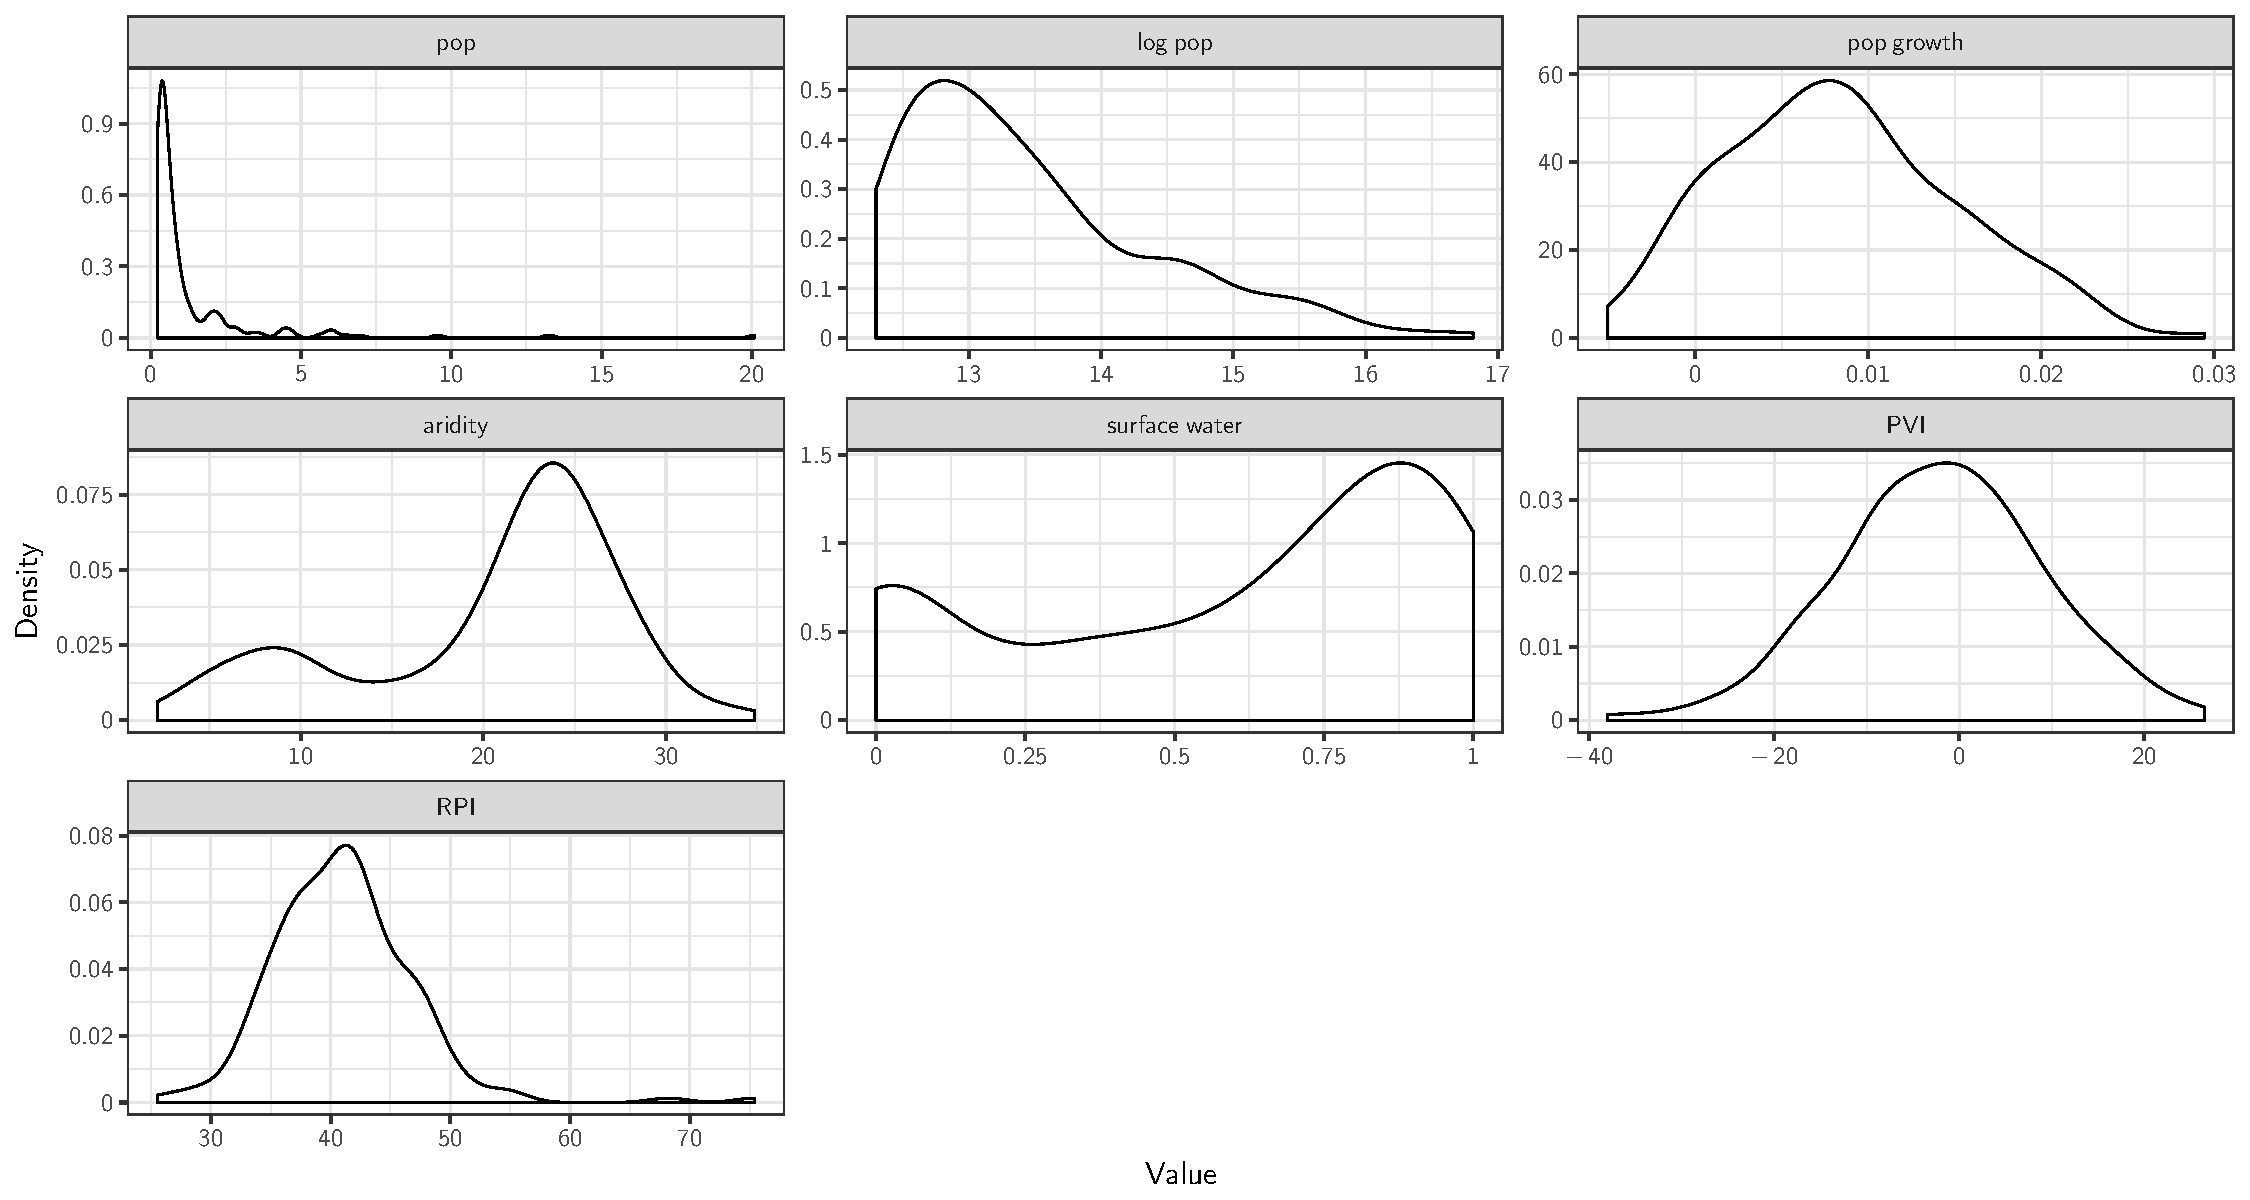
\includegraphics[width=6in]{figures_si/msa_vars_distribution-1} \caption[Kernel-density distribution of MSA-level covariates]{Kernel-density distribution of MSA-level covariates. Population in millions and RPI in thousands of chained 2009 dollars.}\label{fig:msa_vars_distribution}
\end{figure}





% jg_tex_chunk_hook

\begin{figure}
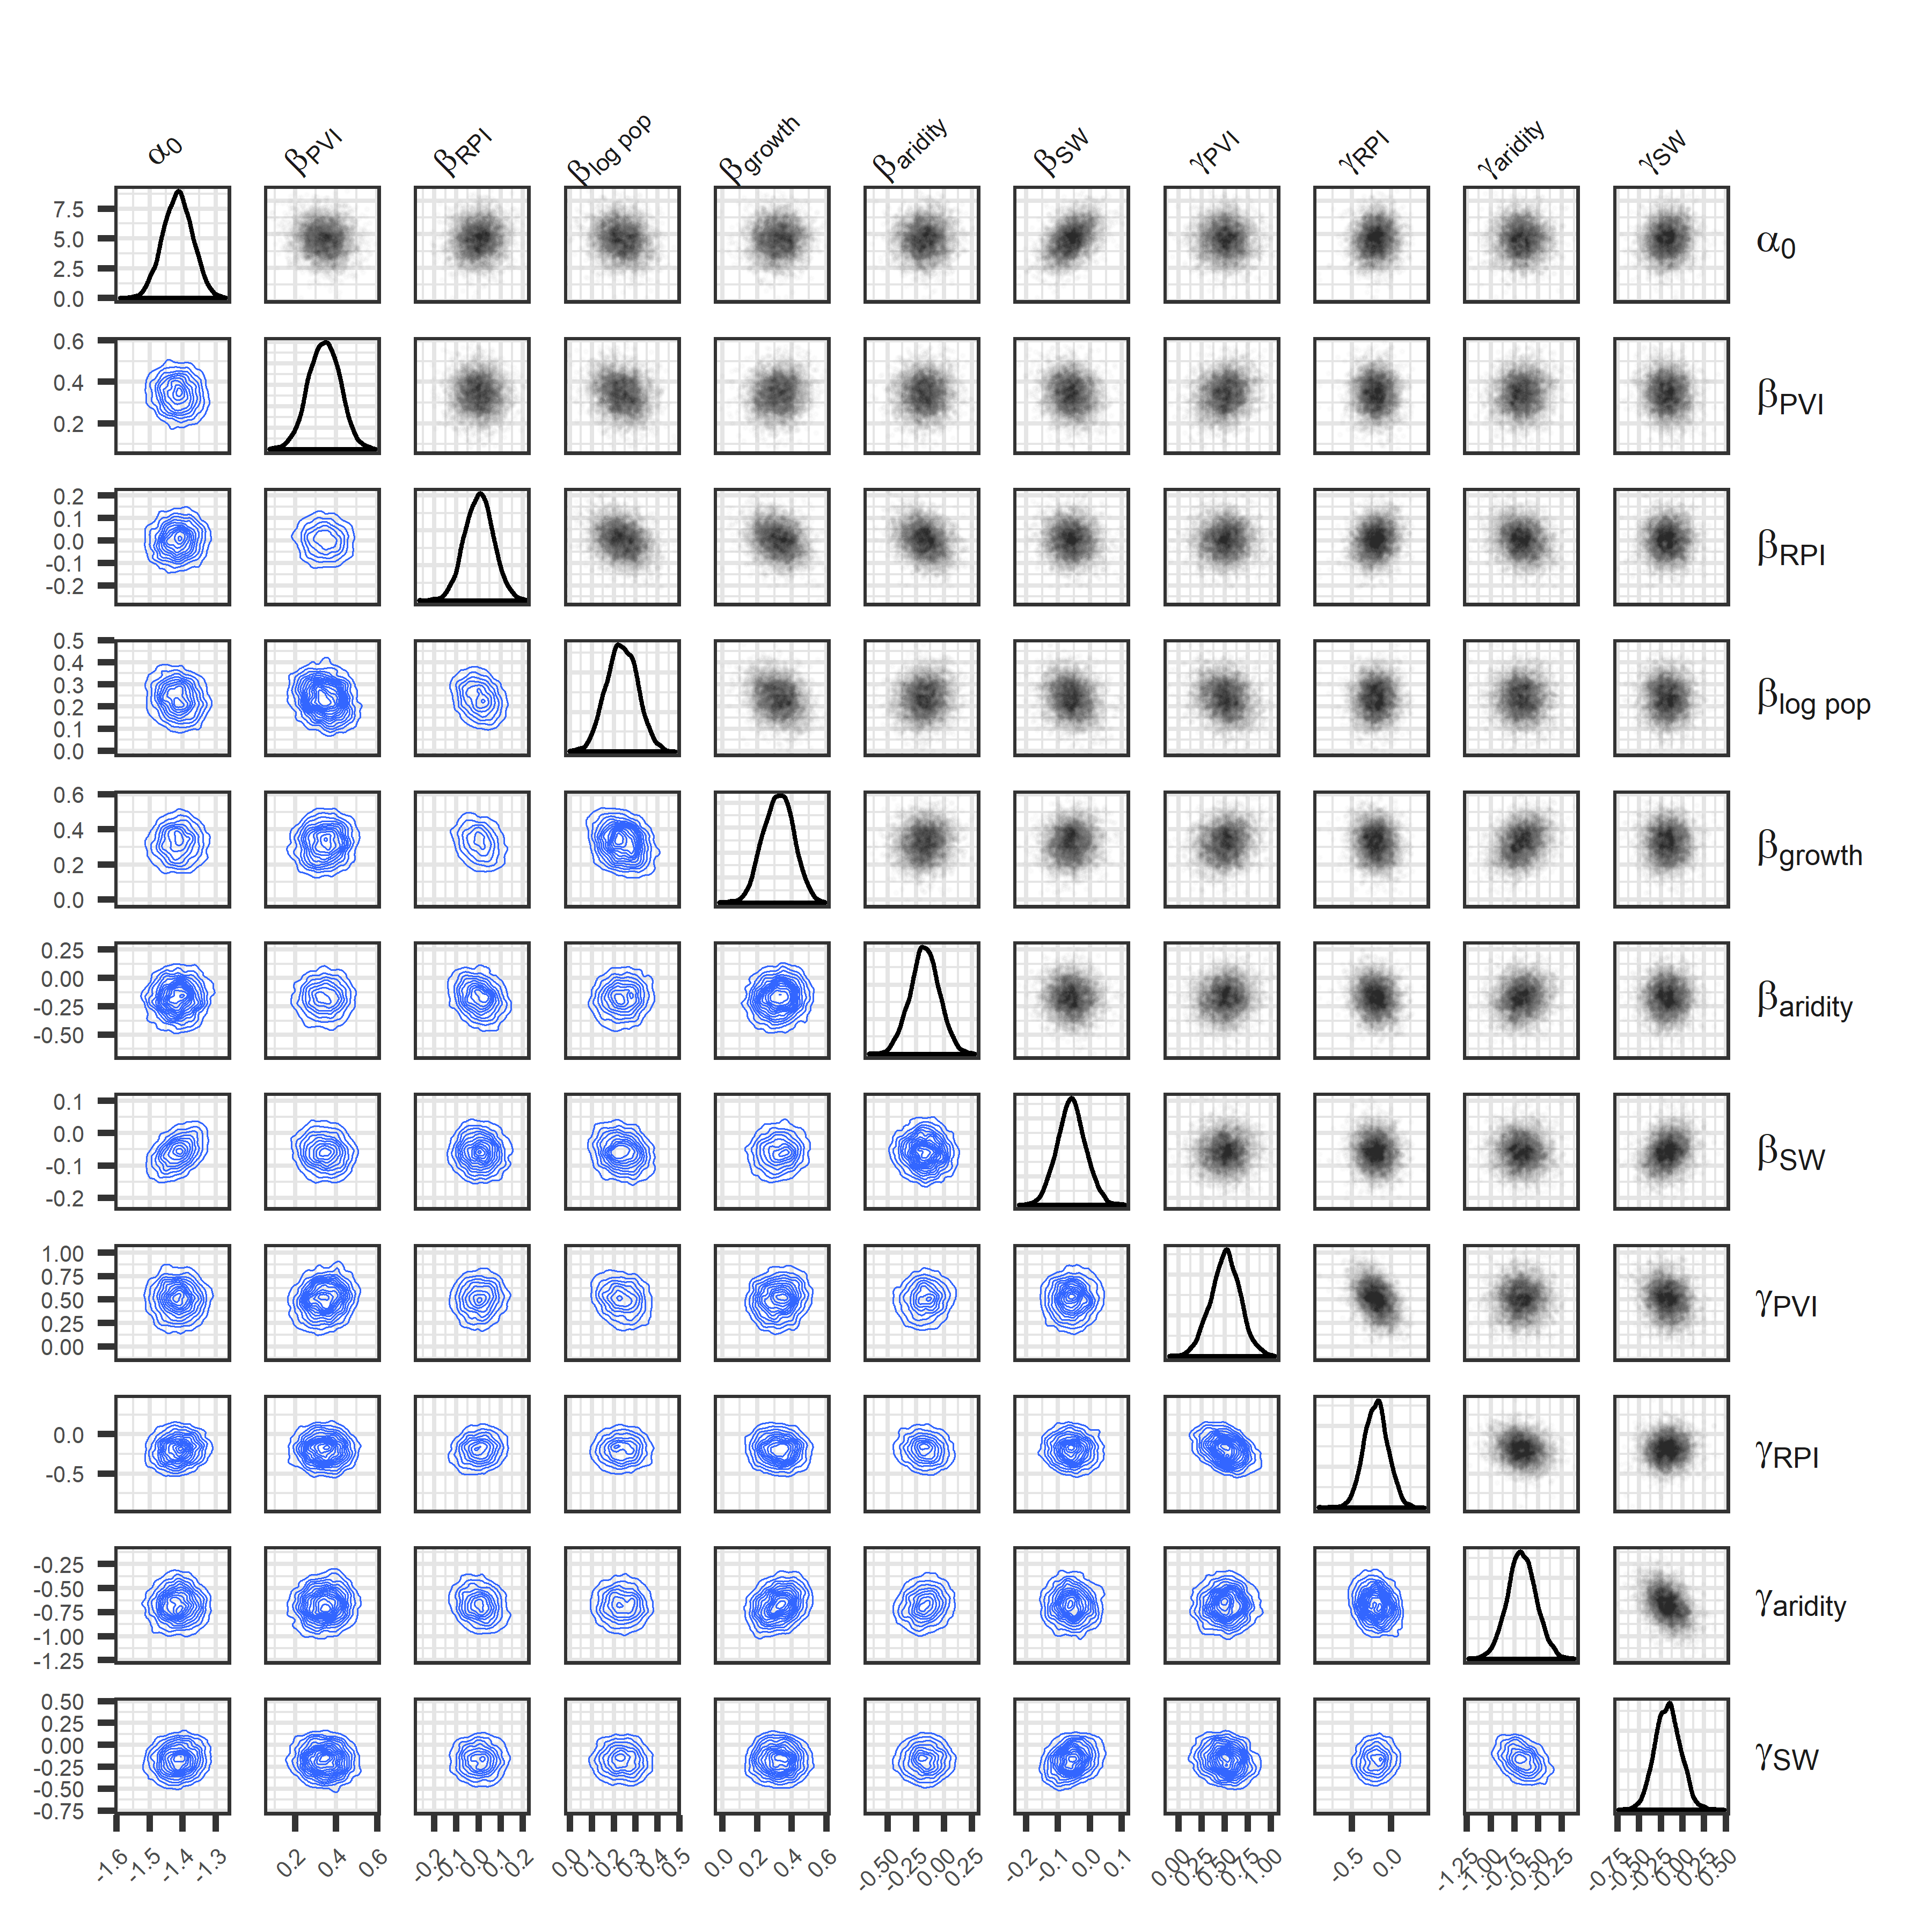
\includegraphics[width=6.25in]{figures_si/vwci_pairs_plot-1} \caption[Correlation plot of posterior probability distribution of regression coefficients $\alpha$, $\beta$, and $\gamma$ for VWCI]{Correlation plot of posterior probability distribution of regression coefficients $\alpha$, $\beta$, and $\gamma$ for VWCI. The diagonal panels show the probability density for each coefficient, panels in the upper triangle show scatterplots of 4000 HMC samples, and panels in the lower triangle show joint probability density contours corresponding to the scatterplot in the upper triangle. Slight correlations are apparent, as between $\gamma_{\text{aridity}}$ and $\gamma_{\text{SW}}$, $\gamma_{\text{PVI}}$ and $\gamma_{\text{RPI}}$, and $\beta_{\text{SW}}$ and $\alpha_0$, but these are small enough not to pose problems apart from slightly increasing the uncertainty in the parameter estimates.}\label{fig:vwci_pairs_plot}
\end{figure}



% jg_tex_chunk_hook

\begin{figure}
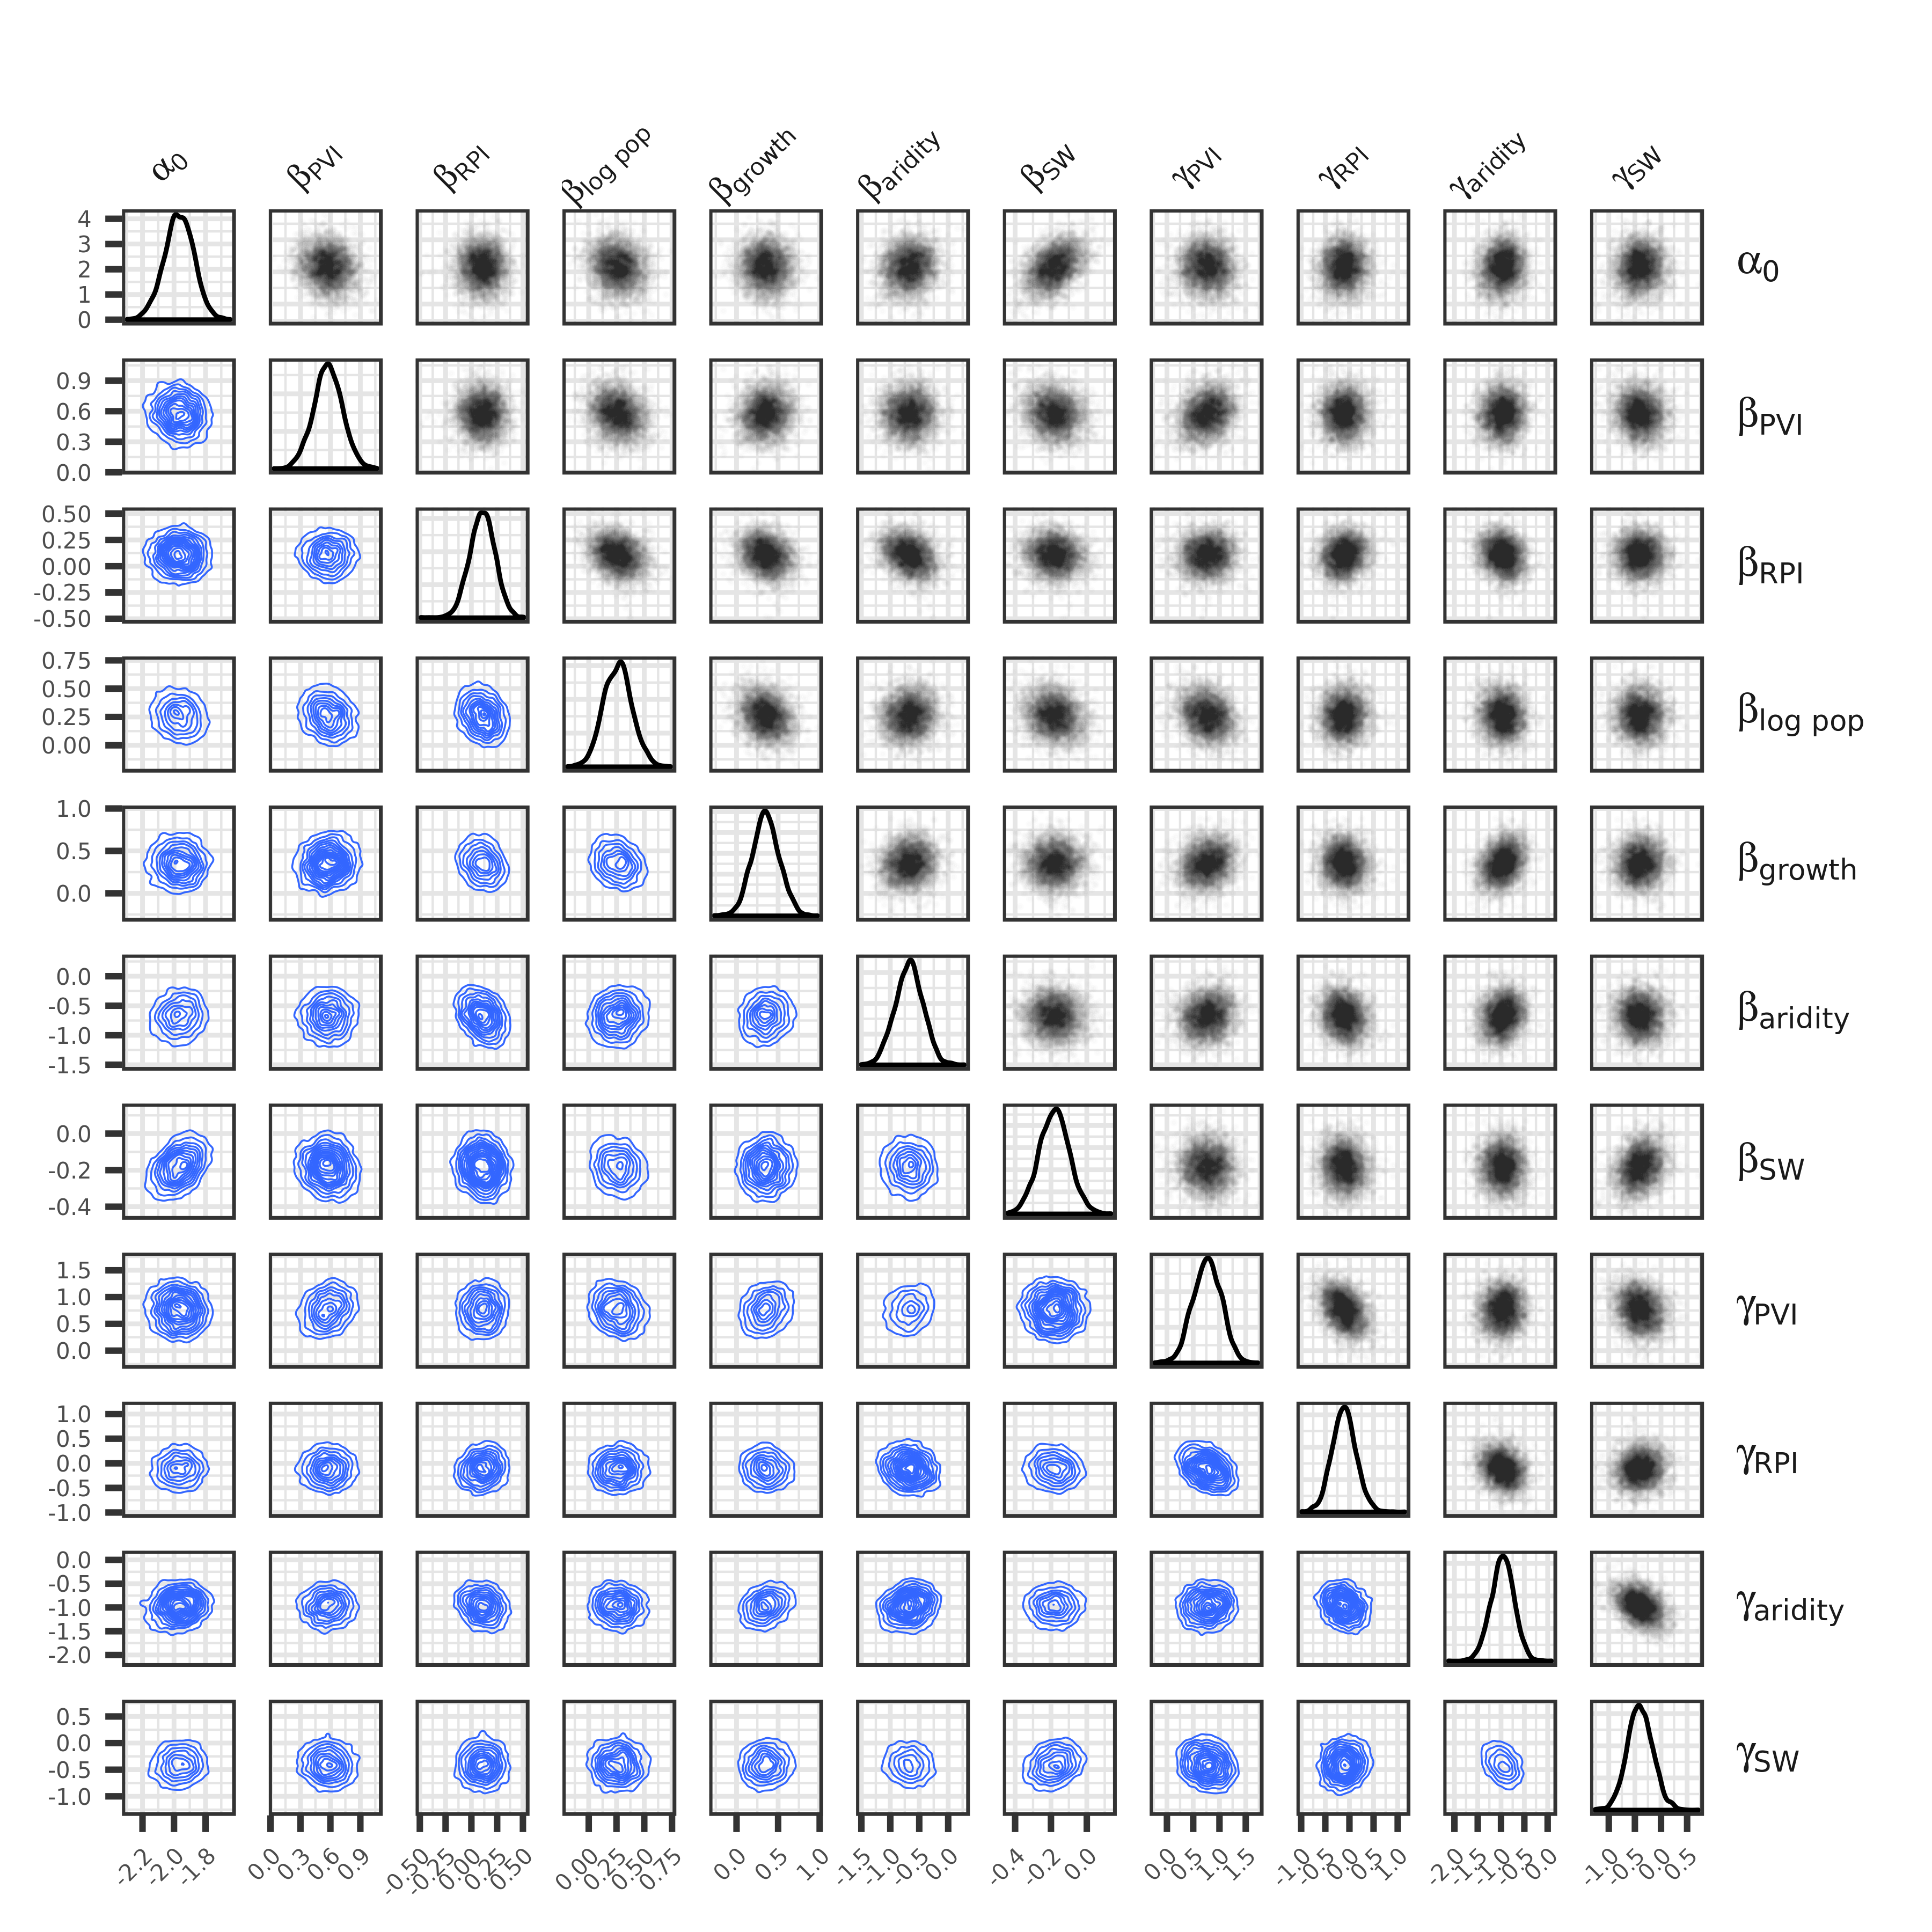
\includegraphics[width=6.25in]{figures_si/req_pairs_plot-1} \caption[Correlation plot of posterior probability distribution of regression coefficients $\alpha$, $\beta$, and $\gamma$ for requirements]{Correlation plot of posterior probability distribution of regression coefficients $\alpha$, $\beta$, and $\gamma$ for requirements.}\label{fig:req_pairs_plot}
\end{figure}



% jg_tex_chunk_hook

\begin{figure}
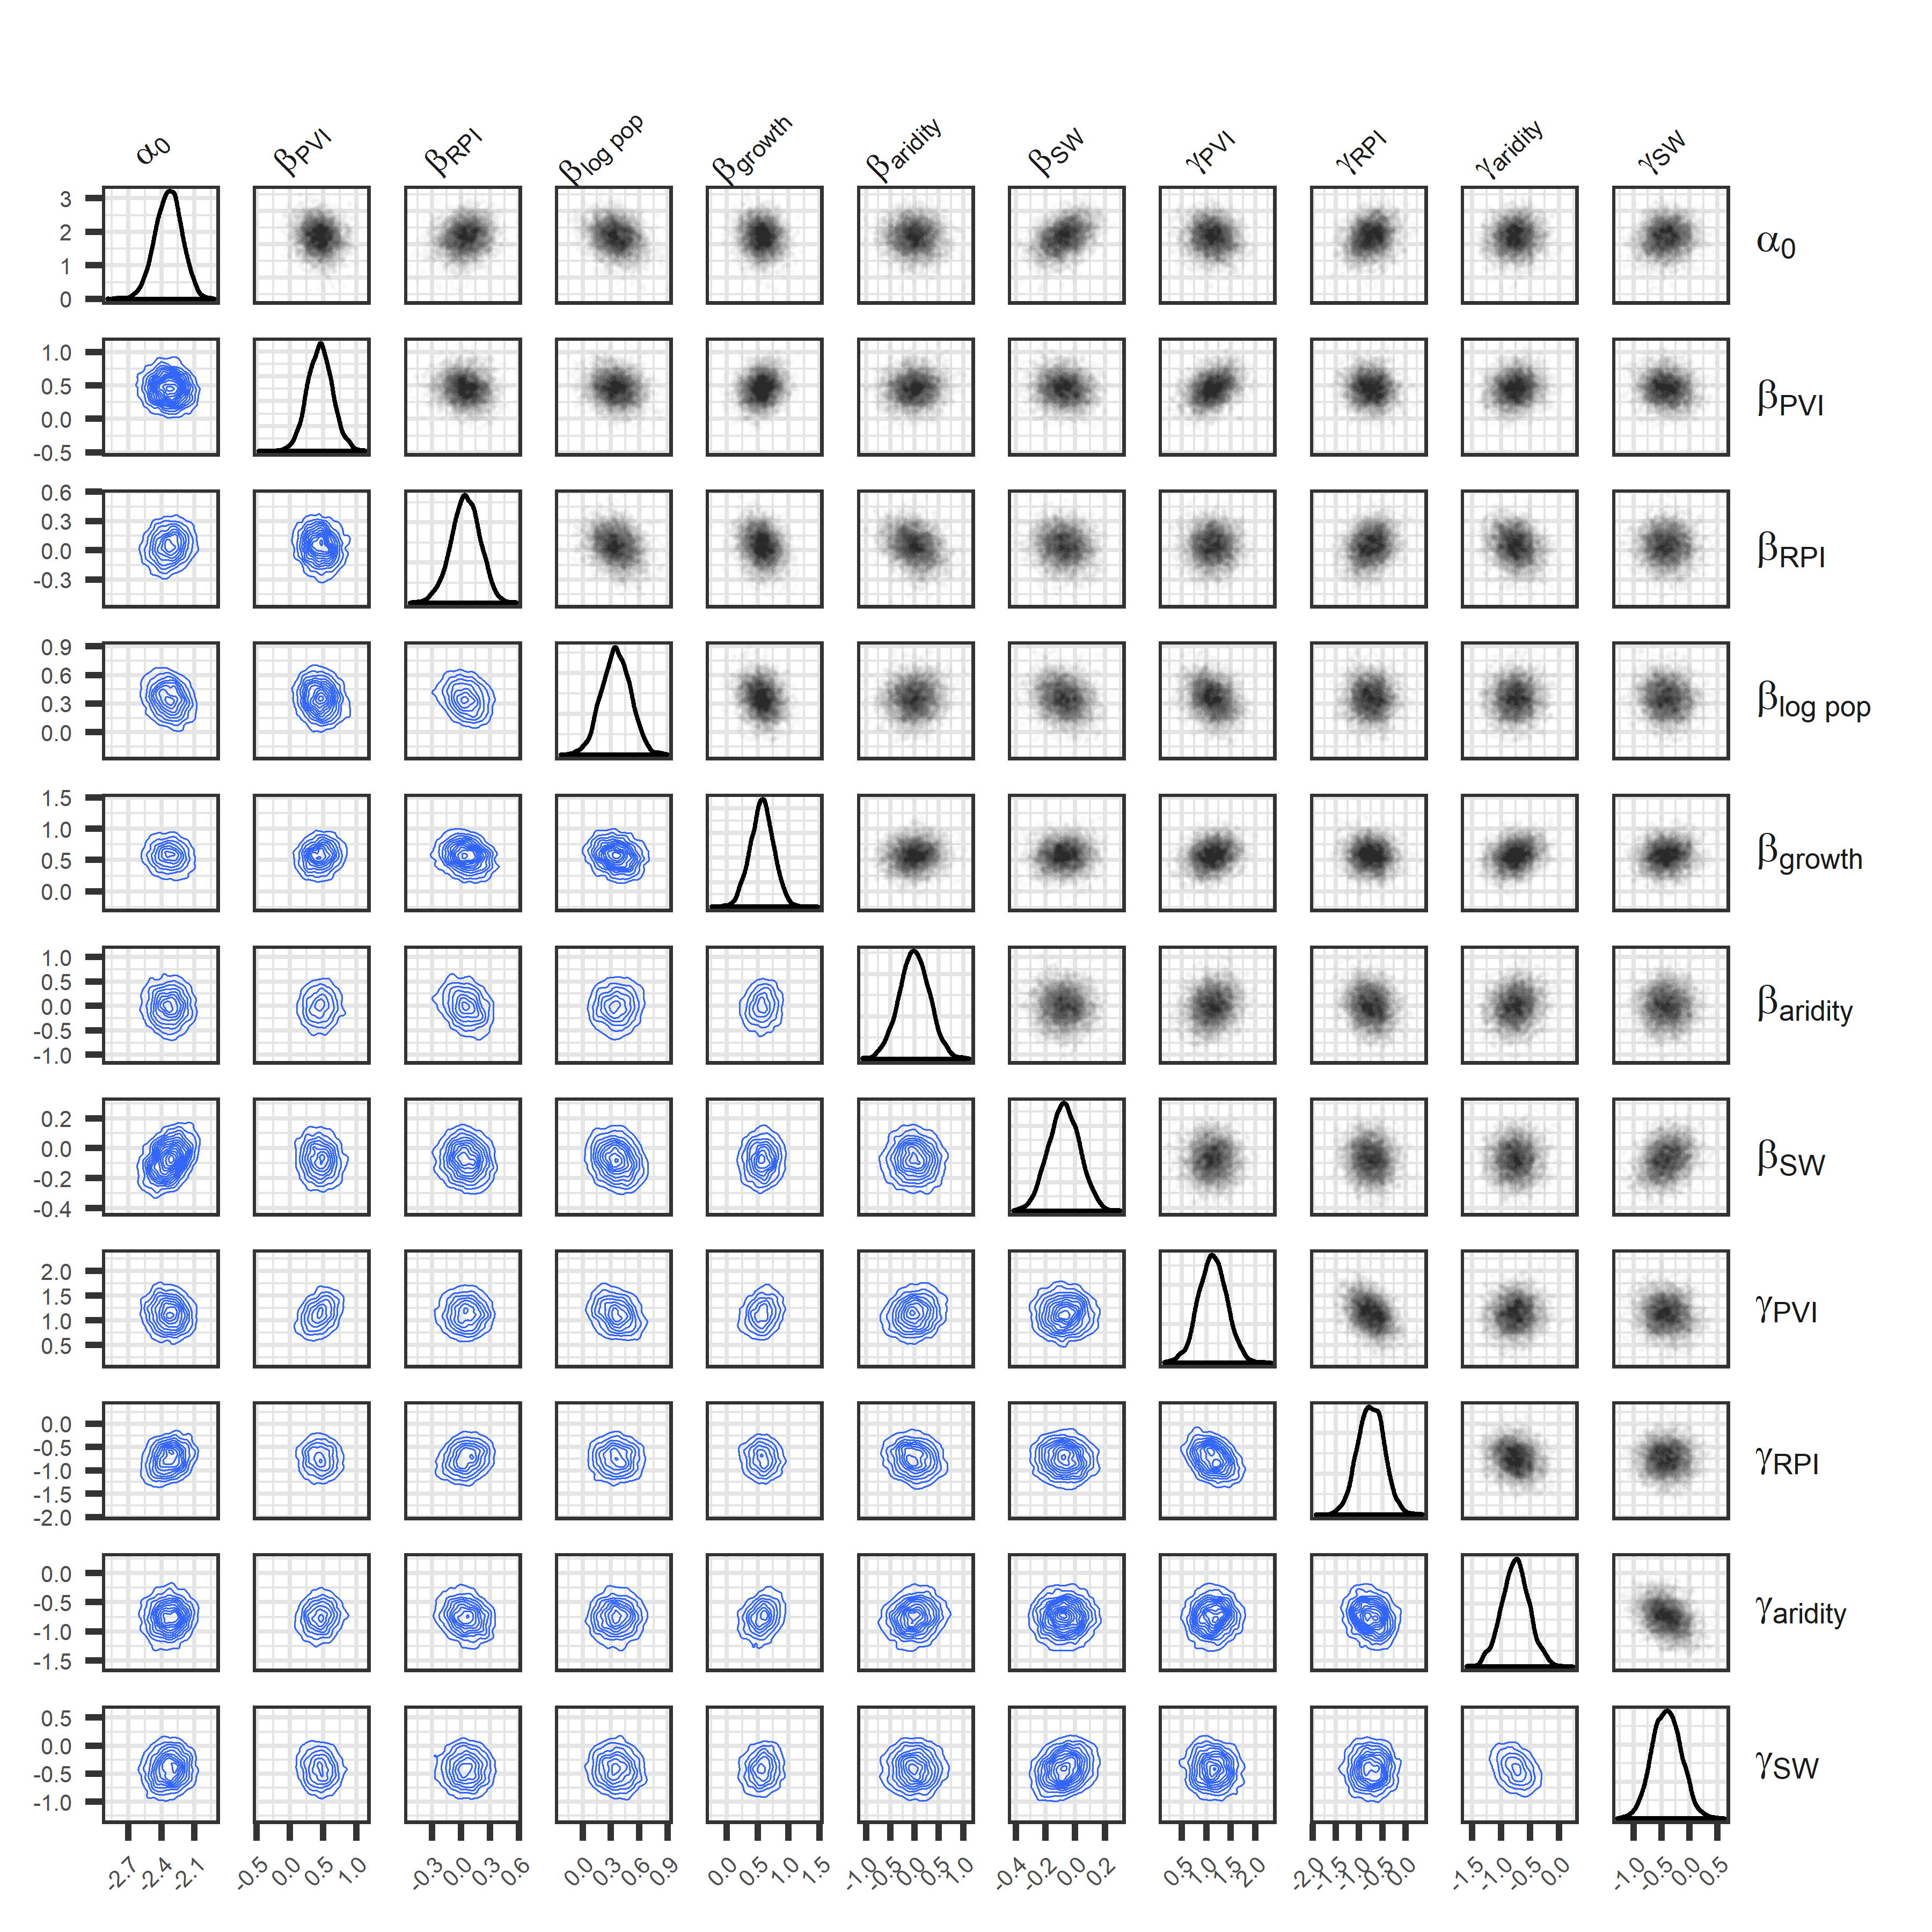
\includegraphics[width=6.25in]{figures_si/reb_pairs_plot-1} \caption[Correlation plot of posterior probability distribution of regression coefficients $\alpha$, $\beta$, and $\gamma$ for rebates]{Correlation plot of posterior probability distribution of regression coefficients $\alpha$, $\beta$, and $\gamma$ for rebates.}\label{fig:reb_pairs_plot}
\end{figure}





% jg_tex_chunk_hook

\begin{figure}
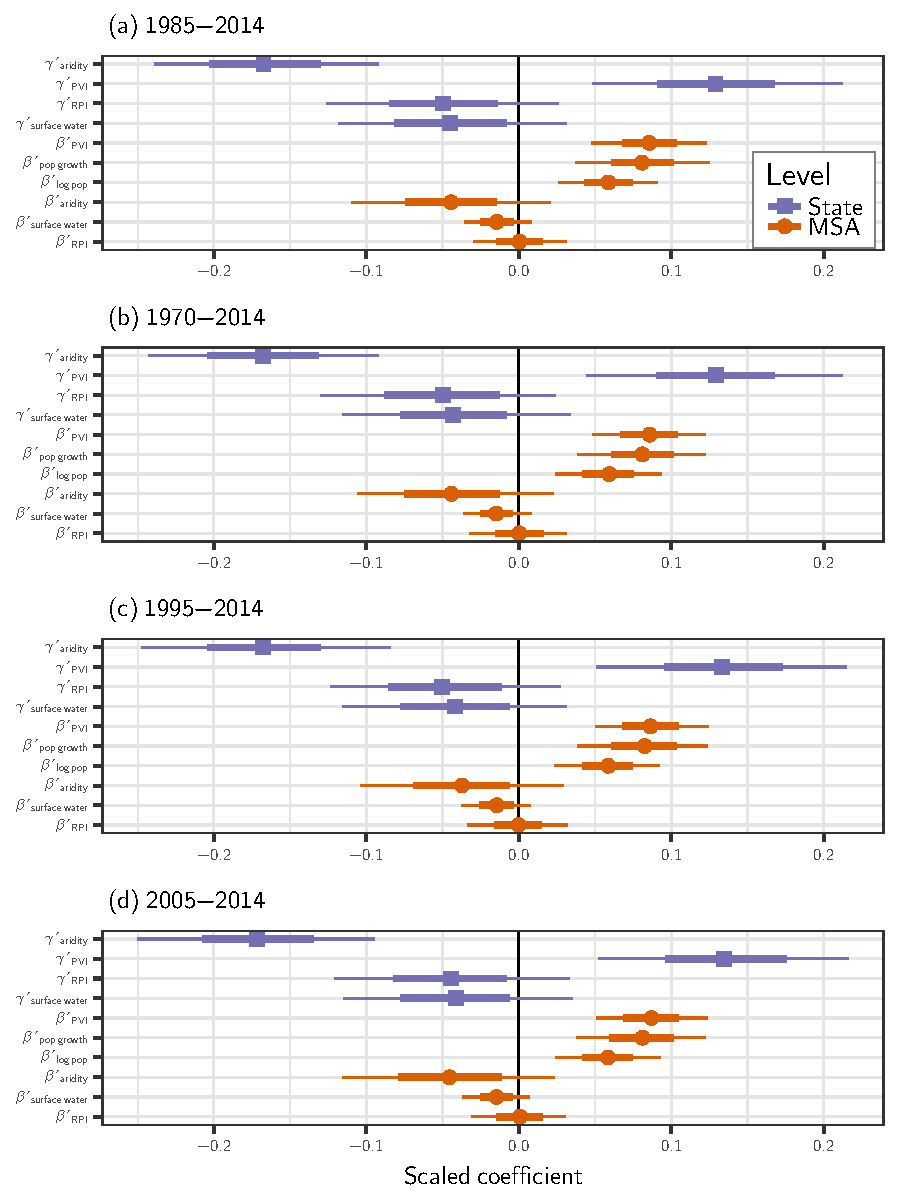
\includegraphics[width=6.25in]{figures_si/vwci_years_cat_plots-1} \caption[Regression coefficients for VWCI, averaging state and MSA aridity over different intervals]{Regression coefficients for VWCI, averaging state and MSA aridity over different intervals.}\label{fig:vwci_years_cat_plots}
\end{figure}



% jg_tex_chunk_hook

\begin{figure}
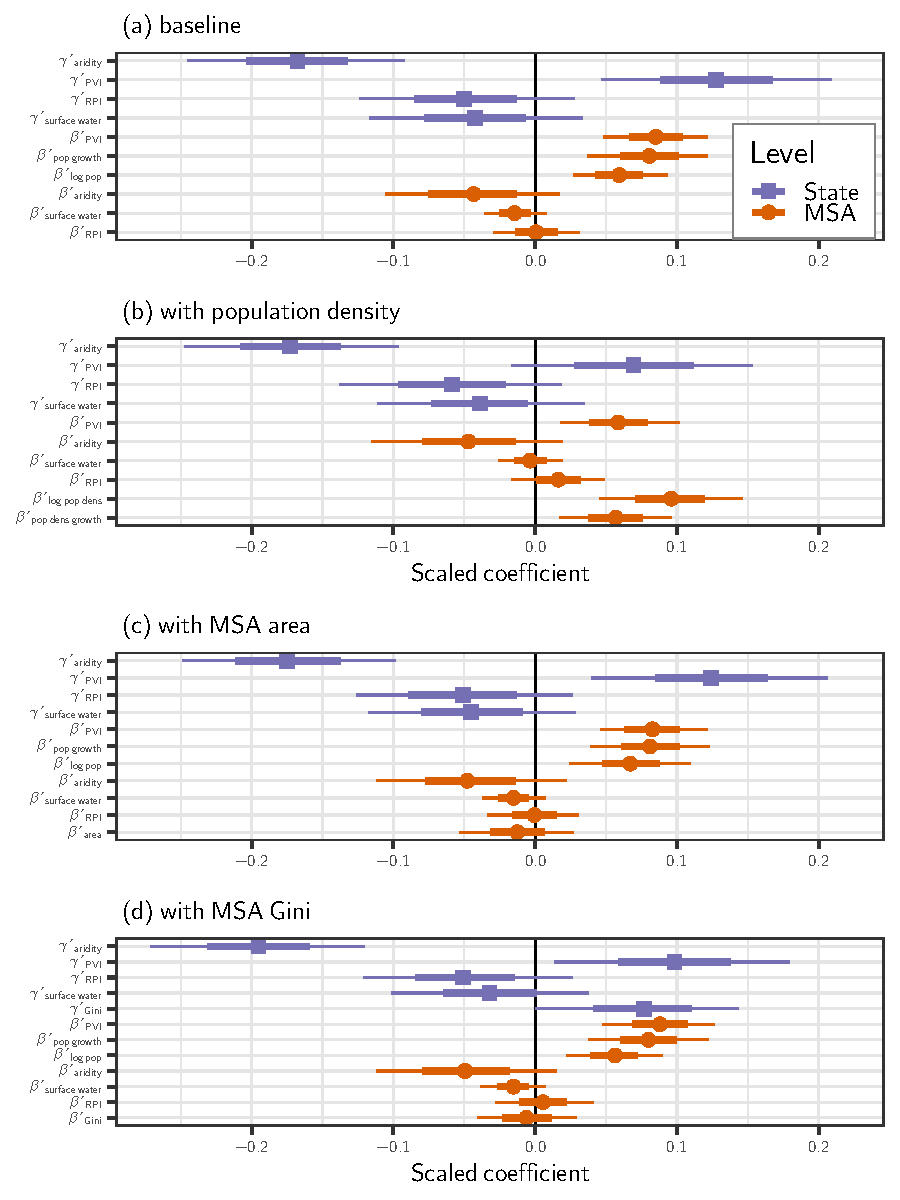
\includegraphics[width=6.25in]{figures_si/vwci_vars_cat_plots-1} \caption[Regression coefficients for VWCI, with different covariates]{Regression coefficients for VWCI, with different covariates.}\label{fig:vwci_vars_cat_plots}
\end{figure}



% jg_tex_chunk_hook

\begin{figure}
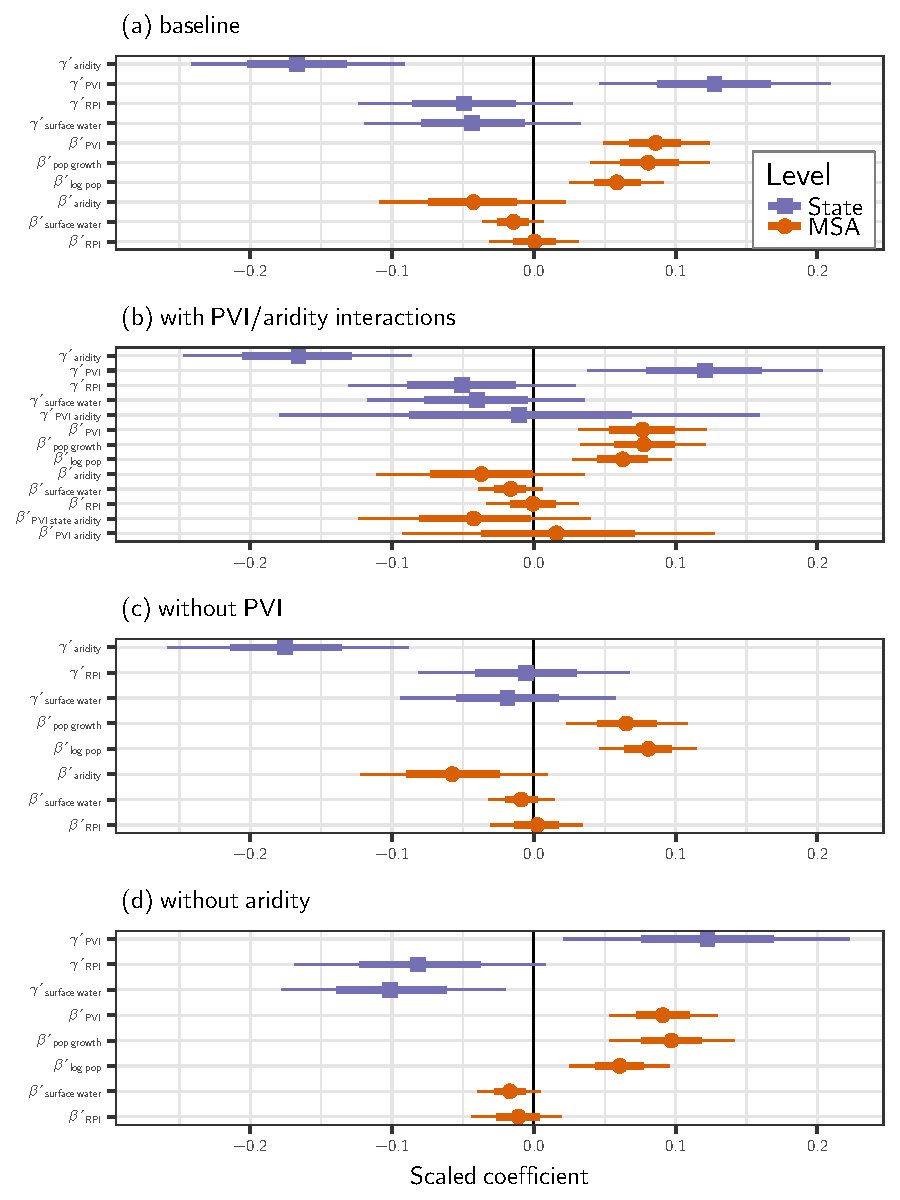
\includegraphics[width=6.25in]{figures_si/vwci_pvi_cat_plots-1} \caption[Regression coefficients for VWCI, with different covariates]{Regression coefficients for VWCI, with different covariates.}\label{fig:vwci_pvi_cat_plots}
\end{figure}




% jg_tex_chunk_hook

\begin{figure}
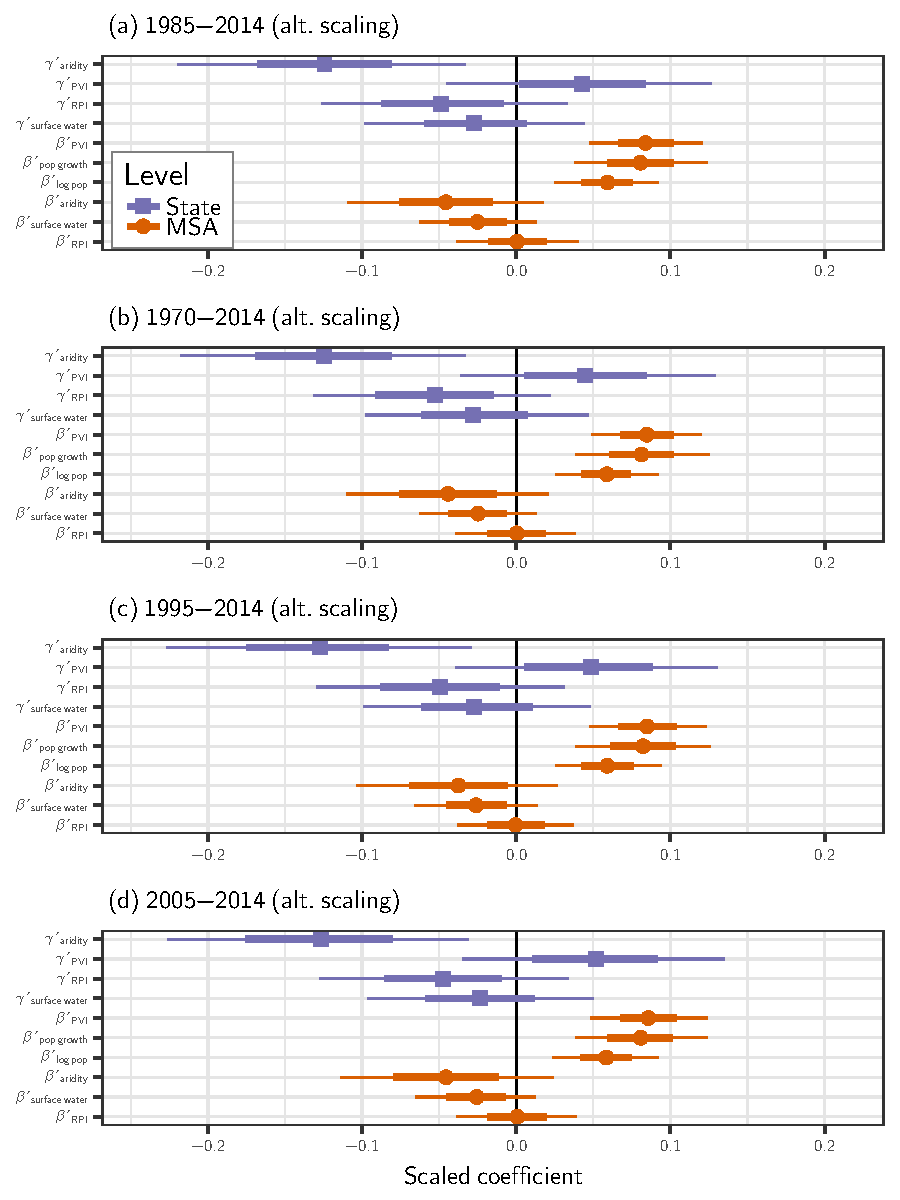
\includegraphics[width=6.25in]{figures_si/pooled_vwci_years_cat_plots-1} \caption[Regression coefficients for VWCI, averaging state and MSA aridity over different intervals, using alternative scaling of MSA-level variables]{Regression coefficients for VWCI, averaging state and MSA aridity over different intervals, using alternative scaling of MSA-level variables.}\label{fig:pooled_vwci_years_cat_plots}
\end{figure}



% jg_tex_chunk_hook

\begin{figure}
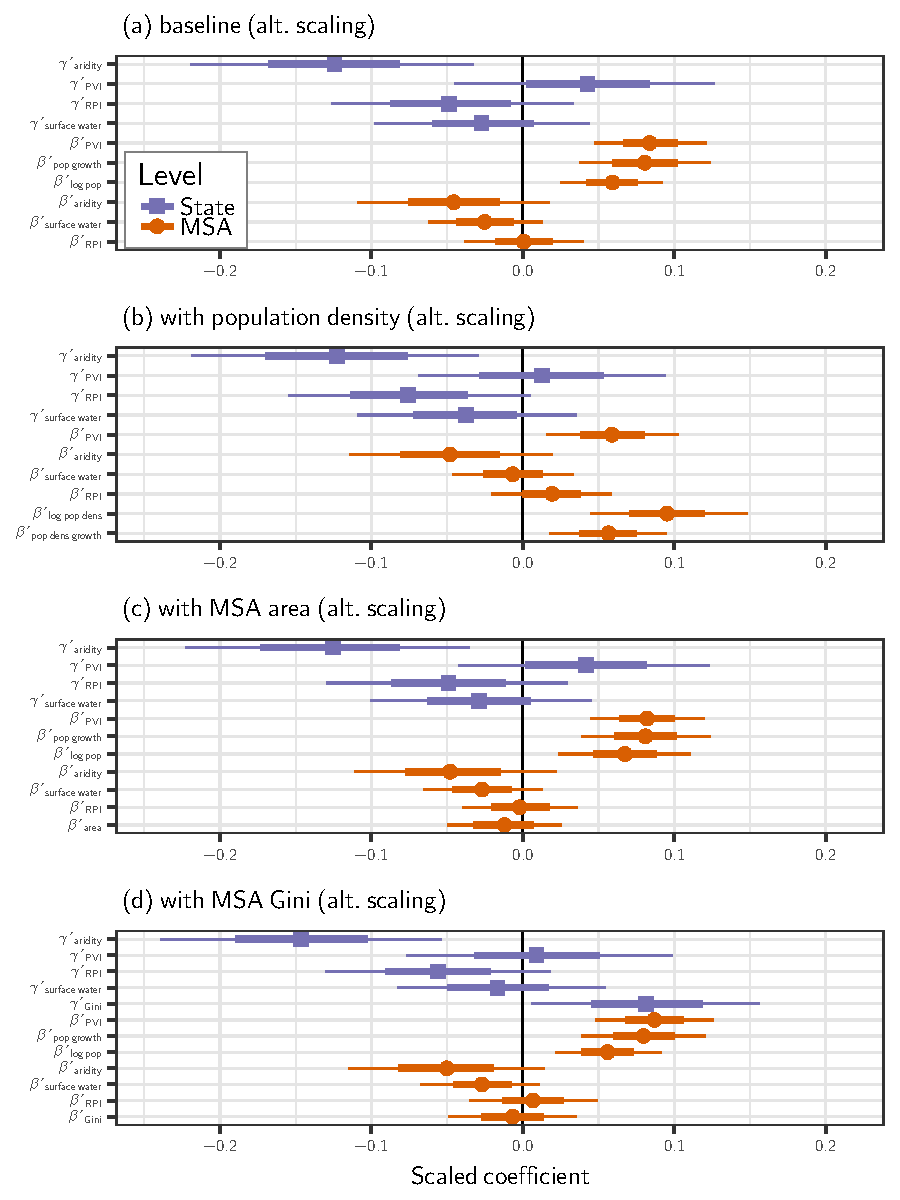
\includegraphics[width=6.25in]{figures_si/pooled_vwci_vars_cat_plots-1} \caption[Regression coefficients for VWCI, with different covariates, using alternative scaling of MSA-level variables]{Regression coefficients for VWCI, with different covariates, using alternative scaling of MSA-level variables.}\label{fig:pooled_vwci_vars_cat_plots}
\end{figure}



% jg_tex_chunk_hook

\begin{figure}
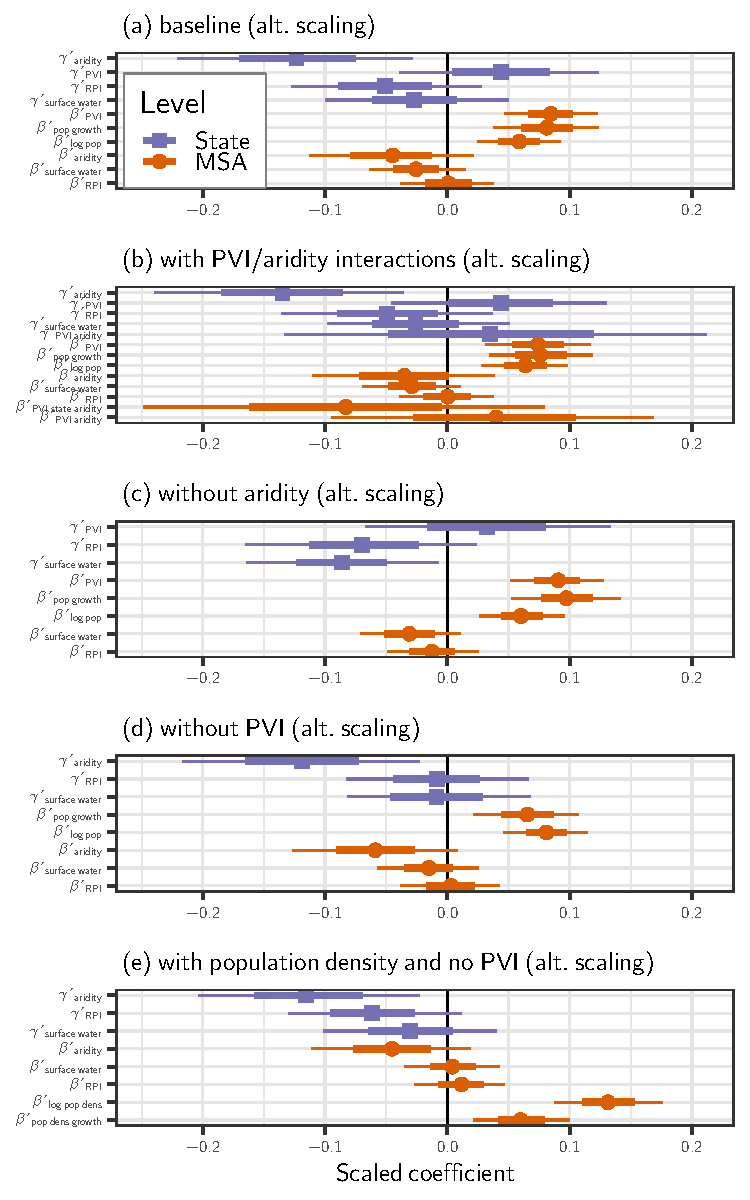
\includegraphics[width=6.25in]{figures_si/pooled_vwci_pvi_cat_plots-1} \caption[Regression coefficients for VWCI, with different covariates, using alternative scaling of MSA-level variables]{Regression coefficients for VWCI, with different covariates, using alternative scaling of MSA-level variables.}\label{fig:pooled_vwci_pvi_cat_plots}
\end{figure}



\clearpage
\section{Tables S1--S17}
\subsection*{Table S1 Caption}
\begin{table}[H]
\centering
Large Tables are available at \url{https://doi.org/10.6084/m9.figshare.5714944}
\caption{Conservation scores and covariates for  cities: VWCI = Vanderbilt Water Conservation Index (total \# of conservation measures), Req.\ = \# requirements, Reb.\ = \# rebates, PVI = Cook Partisan Voting Index, Aridity = K\"oppen aridity index, RPI\ = per-capita real personal income (thousands of regionally adjusted chained 2009 dollars), Pop.\ = population (thousands), Growth = population growth rate (2010--2014), Surf.\ W.\ = surface-water fraction.}
\label{tab:vwci}
\end{table}

\subsection*{Table S2 Caption}
\begin{table}[H]
\centering
Large Tables are available at \url{https://doi.org/10.6084/m9.figshare.5714944}
\caption{State-level covariates: PVI = Cook Partisan Voting Index, RPI = per-capita real personal income (thousands of regionally-adjusted chained 2009 dollars), Aridity = the K\"oppen aridity index, Surf.\ W.\ = the surface-water fraction.}
\label{tab:state}
\end{table}



\subsection*{Table S3}
% latex table generated in R 3.5.0 by xtable 1.8-2 package
% Wed May 16 00:18:48 2018
\begin{table}[H]
\centering
\begingroup\small
\begin{tabular}{p{3in}rrrr}
  \hline
Model & LOO-IC & $\text{s.e.}_{\text{IC}}$ & $\text{ELPD}_{\text{\scshape{loo}}}$ & $\text{s.e.}_{\text{ELPD}}$ \\ 
  \hline
hierarchical beta--binomial: 1995--2014 & 1248.4 & 20.3 & -624.2 & 10.1 \\ 
  hierarchical beta--binomial: 1985--2014 & 1248.6 & 20.5 & -624.3 & 10.3 \\ 
  hierarchical beta--binomial: 1970--2014 & 1249.0 & 20.5 & -624.5 & 10.2 \\ 
  hierarchical beta--binomial: 2005--2014 & 1250.2 & 20.6 & -625.1 & 10.3 \\ 
  hierarchical binomial: 1985--2014 & 1328.3 & 43.9 & -664.1 & 22.0 \\ 
  hierarchical binomial: 1995--2014 & 1328.7 & 43.8 & -664.4 & 21.9 \\ 
  hierarchical binomial: 2005--2014 & 1329.6 & 43.6 & -664.8 & 21.8 \\ 
  hierarchical binomial: 1970--2014 & 1332.6 & 44.2 & -666.3 & 22.1 \\ 
  single-level binomial: 2005--2014 & 1584.3 & 73.5 & -792.2 & 36.7 \\ 
  single-level binomial: 1985--2014 & 1598.3 & 76.5 & -799.1 & 38.2 \\ 
  single-level binomial: 1970--2014 & 1598.6 & 76.6 & -799.3 & 38.3 \\ 
  single-level binomial: 1995--2014 & 1614.9 & 78.6 & -807.4 & 39.3 \\ 
  single-level beta--binomial: 2005--2014 & 1715.9 & 88.5 & -857.9 & 44.2 \\ 
  single-level beta--binomial: 1970--2014 & 1733.9 & 91.7 & -866.9 & 45.8 \\ 
  single-level beta--binomial: 1985--2014 & 1734.9 & 91.7 & -867.4 & 45.8 \\ 
  single-level beta--binomial: 1995--2014 & 1757.5 & 94.4 & -878.7 & 47.2 \\ 
   \hline
\end{tabular}
\endgroup
\caption[Model comparison: LOO (climatological interval).]{Comparing different climatological averaging periods and models: LOO = leave-one-out cross-validation, LOO-IC = LOO information criterion, ELPD = expected log pointwise predictive density, and s.e. indicates the standard error of estimates of quantities. Lower values of the information criteria and greater (less negative) values of ELPD indicate superior model performance. Models are labelled by the time-period for averaging aridity and the structure of the statistical model.} 
\label{tab:loo.years}
\end{table}

\subsection*{Table S4}
% latex table generated in R 3.5.0 by xtable 1.8-2 package
% Wed May 16 00:18:48 2018
\begin{table}[H]
\centering
\begingroup\small
\begin{tabular}{p{3in}rrrr}
  \hline
Model & LOO-IC & $\text{s.e.}_{\text{IC}}$ & $\text{ELPD}_{\text{\scshape{loo}}}$ & $\text{s.e.}_{\text{ELPD}}$ \\ 
  \hline
hierarchical beta--binomial: baseline & 1248.6 & 20.5 & -624.3 & 10.3 \\ 
  hierarchical beta--binomial: with MSA Gini coefficient & 1251.3 & 20.2 & -625.6 & 10.1 \\ 
  hierarchical beta--binomial: without aridity & 1253.6 & 20.8 & -626.8 & 10.4 \\ 
  hierarchical beta--binomial: with MSA area & 1253.7 & 20.7 & -626.9 & 10.4 \\ 
  hierarchical beta--binomial: with PVI/aridity interactions & 1254.2 & 21.4 & -627.1 & 10.7 \\ 
  hierarchical beta--binomial: with pop.\ density & 1261.4 & 23.0 & -630.7 & 11.5 \\ 
  hierarchical beta--binomial: with pop.\ density and no PVI & 1266.4 & 23.4 & -633.2 & 11.7 \\ 
  hierarchical beta--binomial: without PVI & 1269.0 & 21.3 & -634.5 & 10.7 \\ 
  hierarchical binomial: baseline & 1328.3 & 43.9 & -664.1 & 22.0 \\ 
  hierarchical binomial: without aridity & 1331.0 & 44.0 & -665.5 & 22.0 \\ 
  hierarchical binomial: with MSA Gini coefficient & 1334.5 & 43.9 & -667.2 & 22.0 \\ 
  hierarchical binomial: with PVI/aridity interactions & 1335.6 & 46.2 & -667.8 & 23.1 \\ 
  hierarchical binomial: with MSA area & 1338.0 & 44.3 & -669.0 & 22.2 \\ 
  hierarchical binomial: with pop.\ density & 1371.9 & 53.9 & -685.9 & 26.9 \\ 
  hierarchical binomial: without PVI & 1385.3 & 50.6 & -692.7 & 25.3 \\ 
  hierarchical binomial: with pop.\ density and no PVI & 1390.9 & 57.5 & -695.5 & 28.7 \\ 
   \hline
\end{tabular}
\endgroup
\caption[Model comparison: LOO (covariates) for hierarchical regressions.]{Comparing different models and sets of covariates with LOO-IC for hierarchical regressions. Models are labelled by the covariates that differ from the baseline case and the baseline and by the structure of the statistical model.} 
\label{tab:loo.vars}
\end{table}

\subsection*{Table S5}
% latex table generated in R 3.5.0 by xtable 1.8-2 package
% Wed May 16 00:18:48 2018
\begin{table}[H]
\centering
\begingroup\small
\begin{tabular}{p{3in}rrrr}
  \hline
Model & LOO-IC & $\text{s.e.}_{\text{IC}}$ & $\text{ELPD}_{\text{\scshape{loo}}}$ & $\text{s.e.}_{\text{ELPD}}$ \\ 
  \hline
single-level binomial: with PVI/aridity interactions & 1591.4 & 76.8 & -795.7 & 38.4 \\ 
  single-level binomial: with MSA Gini coefficient & 1592.7 & 78.6 & -796.4 & 39.3 \\ 
  single-level binomial: baseline & 1598.3 & 76.5 & -799.1 & 38.2 \\ 
  single-level binomial: with MSA area & 1601.9 & 76.6 & -801.0 & 38.3 \\ 
  single-level binomial: with pop.\ density & 1679.0 & 87.2 & -839.5 & 43.6 \\ 
  single-level binomial: without PVI & 1683.8 & 89.1 & -841.9 & 44.6 \\ 
  single-level binomial: with pop.\ density and no PVI & 1692.5 & 89.0 & -846.2 & 44.5 \\ 
  single-level beta--binomial: baseline & 1734.9 & 91.7 & -867.4 & 45.8 \\ 
  single-level beta--binomial: with MSA Gini coefficient & 1750.4 & 96.9 & -875.2 & 48.4 \\ 
  single-level beta--binomial: with PVI/aridity interactions & 1773.6 & 100.0 & -886.8 & 50.0 \\ 
  single-level beta--binomial: with MSA area & 1797.4 & 106.3 & -898.7 & 53.2 \\ 
  single-level beta--binomial: with pop.\ density and no PVI & 1821.1 & 97.9 & -910.6 & 48.9 \\ 
  single-level beta--binomial: without PVI & 1824.1 & 100.9 & -912.0 & 50.5 \\ 
  single-level beta--binomial: with pop.\ density & 1828.1 & 99.8 & -914.0 & 49.9 \\ 
  single-level binomial: without aridity & 1850.9 & 112.0 & -925.4 & 56.0 \\ 
  single-level beta--binomial: without aridity & 2068.9 & 137.1 & -1034.5 & 68.5 \\ 
   \hline
\end{tabular}
\endgroup
\caption[Model comparison: LOO (covariates) for single-level regressions.]{Model Comparison with LOO-IC for single-level regressions and different sets of covariates.} 
\label{tab:loo.vars}
\end{table}

\subsection*{Table S6}
% latex table generated in R 3.5.0 by xtable 1.8-2 package
% Wed May 16 00:18:48 2018
\begin{table}[H]
\centering
\begingroup\small
\begin{tabular}{p{3in}rrrr}
  \hline
Model & WAIC & $\text{s.e.}_{\text{IC}}$ & $\text{ELPD}_{\text{\scshape{waic}}}$ & $\text{s.e.}_{\text{ELPD}}$ \\ 
  \hline
hierarchical beta--binomial: 1985--2014 & 1244.3 & 20.2 & -622.2 & 10.1 \\ 
  hierarchical beta--binomial: 1970--2014 & 1244.5 & 20.1 & -622.2 & 10.0 \\ 
  hierarchical beta--binomial: 1995--2014 & 1244.7 & 20.0 & -622.3 & 10.0 \\ 
  hierarchical beta--binomial: 2005--2014 & 1245.3 & 20.1 & -622.7 & 10.1 \\ 
  hierarchical binomial: 2005--2014 & 1317.6 & 43.1 & -658.8 & 21.6 \\ 
  hierarchical binomial: 1985--2014 & 1317.7 & 43.5 & -658.9 & 21.7 \\ 
  hierarchical binomial: 1995--2014 & 1317.8 & 43.3 & -658.9 & 21.6 \\ 
  hierarchical binomial: 1970--2014 & 1319.0 & 43.5 & -659.5 & 21.7 \\ 
  single-level binomial: 2005--2014 & 1583.9 & 73.4 & -791.9 & 36.7 \\ 
  single-level binomial: 1985--2014 & 1598.1 & 76.5 & -799.0 & 38.2 \\ 
  single-level binomial: 1970--2014 & 1598.1 & 76.5 & -799.1 & 38.2 \\ 
  single-level binomial: 1995--2014 & 1614.1 & 78.4 & -807.1 & 39.2 \\ 
  single-level beta--binomial: 2005--2014 & 1702.7 & 86.4 & -851.3 & 43.2 \\ 
  single-level beta--binomial: 1970--2014 & 1722.0 & 90.4 & -861.0 & 45.2 \\ 
  single-level beta--binomial: 1985--2014 & 1724.9 & 90.6 & -862.5 & 45.3 \\ 
  single-level beta--binomial: 1995--2014 & 1744.5 & 92.9 & -872.2 & 46.5 \\ 
   \hline
\end{tabular}
\endgroup
\caption[Model comparison: WAIC (climatological interval).]{Model comparison: WAIC = widely applicable information criterion (also known as the Watanabe-Aikake Information Criterion), ELPD = expected log-probability density, and s.e. indicates the standard error of estimates of quantities. Lower values of the information criteria and greater (less negative) values of ELPD indicate superior model performance. Models are labelled by the time-period for averaging aridity and the structure of the statistical model.} 
\label{tab:waic.years}
\end{table}

\subsection*{Table S7}
% latex table generated in R 3.5.0 by xtable 1.8-2 package
% Wed May 16 00:18:48 2018
\begin{table}[H]
\centering
\begingroup\small
\begin{tabular}{p{3in}rrrr}
  \hline
Model & WAIC & $\text{s.e.}_{\text{IC}}$ & $\text{ELPD}_{\text{\scshape{waic}}}$ & $\text{s.e.}_{\text{ELPD}}$ \\ 
  \hline
hierarchical beta--binomial: baseline & 1244.3 & 20.2 & -622.2 & 10.1 \\ 
  hierarchical beta--binomial: without aridity & 1247.7 & 20.2 & -623.9 & 10.1 \\ 
  hierarchical beta--binomial: with MSA Gini coefficient & 1247.8 & 19.9 & -623.9 & 10.0 \\ 
  hierarchical beta--binomial: with MSA area & 1248.0 & 20.2 & -624.0 & 10.1 \\ 
  hierarchical beta--binomial: with PVI/aridity interactions & 1248.7 & 21.0 & -624.4 & 10.5 \\ 
  hierarchical beta--binomial: with pop.\ density & 1258.6 & 22.9 & -629.3 & 11.4 \\ 
  hierarchical beta--binomial: with pop.\ density and no PVI & 1264.1 & 23.3 & -632.0 & 11.6 \\ 
  hierarchical beta--binomial: without PVI & 1265.4 & 21.1 & -632.7 & 10.5 \\ 
  hierarchical binomial: without aridity & 1317.4 & 43.2 & -658.7 & 21.6 \\ 
  hierarchical binomial: baseline & 1317.7 & 43.5 & -658.9 & 21.7 \\ 
  hierarchical binomial: with PVI/aridity interactions & 1322.8 & 45.5 & -661.4 & 22.7 \\ 
  hierarchical binomial: with MSA Gini coefficient & 1322.9 & 43.4 & -661.5 & 21.7 \\ 
  hierarchical binomial: with MSA area & 1323.6 & 43.6 & -661.8 & 21.8 \\ 
  hierarchical binomial: with pop.\ density & 1361.6 & 53.6 & -680.8 & 26.8 \\ 
  hierarchical binomial: without PVI & 1370.9 & 49.8 & -685.5 & 24.9 \\ 
  hierarchical binomial: with pop.\ density and no PVI & 1381.4 & 57.2 & -690.7 & 28.6 \\ 
   \hline
\end{tabular}
\endgroup
\caption[Model comparison: WAIC (alternate covariates) for hierarchical regressions.]{Model comparison with WAIC for hierarchical regressions. Models are labelled by the covariates that differ from the baseline case and by the structure of the statistical model.} 
\label{tab:waic.vars}
\end{table}

\subsection*{Table S8}
% latex table generated in R 3.5.0 by xtable 1.8-2 package
% Wed May 16 00:18:48 2018
\begin{table}[H]
\centering
\begingroup\small
\begin{tabular}{p{3in}rrrr}
  \hline
Model & WAIC & $\text{s.e.}_{\text{IC}}$ & $\text{ELPD}_{\text{\scshape{waic}}}$ & $\text{s.e.}_{\text{ELPD}}$ \\ 
  \hline
single-level binomial: with PVI/aridity interactions & 1590.9 & 76.8 & -795.5 & 38.4 \\ 
  single-level binomial: with MSA Gini coefficient & 1591.8 & 78.4 & -795.9 & 39.2 \\ 
  single-level binomial: baseline & 1598.1 & 76.5 & -799.0 & 38.2 \\ 
  single-level binomial: with MSA area & 1599.3 & 76.1 & -799.6 & 38.1 \\ 
  single-level binomial: with pop.\ density & 1678.7 & 87.2 & -839.4 & 43.6 \\ 
  single-level binomial: without PVI & 1683.7 & 89.1 & -841.9 & 44.6 \\ 
  single-level binomial: with pop.\ density and no PVI & 1692.2 & 89.0 & -846.1 & 44.5 \\ 
  single-level beta--binomial: baseline & 1724.9 & 90.6 & -862.5 & 45.3 \\ 
  single-level beta--binomial: with MSA Gini coefficient & 1732.7 & 95.0 & -866.4 & 47.5 \\ 
  single-level beta--binomial: with PVI/aridity interactions & 1745.9 & 96.4 & -873.0 & 48.2 \\ 
  single-level beta--binomial: with MSA area & 1768.8 & 99.8 & -884.4 & 49.9 \\ 
  single-level beta--binomial: with pop.\ density and no PVI & 1805.5 & 96.3 & -902.8 & 48.2 \\ 
  single-level beta--binomial: without PVI & 1809.0 & 99.4 & -904.5 & 49.7 \\ 
  single-level beta--binomial: with pop.\ density & 1810.6 & 97.6 & -905.3 & 48.8 \\ 
  single-level binomial: without aridity & 1850.6 & 112.0 & -925.3 & 56.0 \\ 
  single-level beta--binomial: without aridity & 2060.8 & 137.6 & -1030.4 & 68.8 \\ 
   \hline
\end{tabular}
\endgroup
\caption[Model comparison: WAIC (alternate covariates) for single-level regressions.]{Model comparison with WAIC for single-level regressions and different sets of covariates.} 
\label{tab:waic.vars}
\end{table}



\subsection*{Table S9}
% latex table generated in R 3.5.0 by xtable 1.8-2 package
% Wed May 16 00:23:29 2018
\begin{table}[H]
\centering
\begingroup\small
\begin{tabular}{p{3in}rrrr}
  \hline
Model & LOO-IC & $\text{s.e.}_{\text{IC}}$ & $\text{ELPD}_{\text{\scshape{loo}}}$ & $\text{s.e.}_{\text{ELPD}}$ \\ 
  \hline
hierarchical beta--binomial: 2005--2014 & 1248.3 & 20.3 & -624.2 & 10.2 \\ 
  hierarchical beta--binomial: 1995--2014 & 1248.6 & 20.4 & -624.3 & 10.2 \\ 
  hierarchical beta--binomial: 1985--2014 & 1248.9 & 20.6 & -624.5 & 10.3 \\ 
  hierarchical beta--binomial: 1970--2014 & 1249.0 & 20.5 & -624.5 & 10.2 \\ 
  hierarchical binomial: 1995--2014 & 1328.3 & 43.8 & -664.1 & 21.9 \\ 
  hierarchical binomial: 1985--2014 & 1329.1 & 44.1 & -664.6 & 22.0 \\ 
  hierarchical binomial: 2005--2014 & 1329.5 & 43.7 & -664.7 & 21.9 \\ 
  hierarchical binomial: 1970--2014 & 1330.8 & 44.3 & -665.4 & 22.1 \\ 
  single-level binomial: 2005--2014 & 1585.9 & 73.7 & -793.0 & 36.9 \\ 
  single-level binomial: 1985--2014 & 1597.7 & 76.3 & -798.8 & 38.2 \\ 
  single-level binomial: 1970--2014 & 1599.6 & 76.7 & -799.8 & 38.3 \\ 
  single-level binomial: 1995--2014 & 1614.8 & 78.4 & -807.4 & 39.2 \\ 
  single-level beta--binomial: 2005--2014 & 1714.9 & 88.9 & -857.5 & 44.5 \\ 
  single-level beta--binomial: 1985--2014 & 1726.8 & 91.6 & -863.4 & 45.8 \\ 
  single-level beta--binomial: 1970--2014 & 1734.5 & 92.0 & -867.3 & 46.0 \\ 
  single-level beta--binomial: 1995--2014 & 1765.4 & 95.6 & -882.7 & 47.8 \\ 
   \hline
\end{tabular}
\endgroup
\caption[Model comparison: LOO (climatological interval using alternative scaling).]{Model comparison with LOO-IC for different climatological averaging periods and models, using the alternative scaling for MSA-level covariates.} 
\label{tab:loo.years}
\end{table}

\subsection*{Table S10}
% latex table generated in R 3.5.0 by xtable 1.8-2 package
% Wed May 16 00:23:29 2018
\begin{table}[H]
\centering
\begingroup\small
\begin{tabular}{p{3in}rrrr}
  \hline
Model & LOO-IC & $\text{s.e.}_{\text{IC}}$ & $\text{ELPD}_{\text{\scshape{loo}}}$ & $\text{s.e.}_{\text{ELPD}}$ \\ 
  \hline
hierarchical beta--binomial: baseline & 1248.9 & 20.6 & -624.5 & 10.3 \\ 
  hierarchical beta--binomial: with MSA area & 1252.5 & 20.6 & -626.3 & 10.3 \\ 
  hierarchical beta--binomial: with MSA Gini coefficient & 1252.6 & 20.3 & -626.3 & 10.2 \\ 
  hierarchical beta--binomial: without aridity & 1252.7 & 20.7 & -626.3 & 10.4 \\ 
  hierarchical beta--binomial: with PVI/aridity interactions & 1254.8 & 21.2 & -627.4 & 10.6 \\ 
  hierarchical beta--binomial: with pop.\ density & 1262.1 & 23.0 & -631.0 & 11.5 \\ 
  hierarchical beta--binomial: with pop.\ density and no PVI & 1266.7 & 23.4 & -633.3 & 11.7 \\ 
  hierarchical beta--binomial: without PVI & 1269.1 & 21.3 & -634.6 & 10.6 \\ 
  hierarchical binomial: baseline & 1329.1 & 44.1 & -664.6 & 22.0 \\ 
  hierarchical binomial: without aridity & 1329.6 & 43.5 & -664.8 & 21.8 \\ 
  hierarchical binomial: with PVI/aridity interactions & 1332.4 & 45.9 & -666.2 & 22.9 \\ 
  hierarchical binomial: with MSA area & 1335.4 & 44.3 & -667.7 & 22.1 \\ 
  hierarchical binomial: with MSA Gini coefficient & 1337.5 & 44.4 & -668.8 & 22.2 \\ 
  hierarchical binomial: with pop.\ density & 1370.5 & 54.1 & -685.3 & 27.0 \\ 
  hierarchical binomial: without PVI & 1380.0 & 49.9 & -690.0 & 25.0 \\ 
  hierarchical binomial: with pop.\ density and no PVI & 1388.7 & 57.4 & -694.3 & 28.7 \\ 
   \hline
\end{tabular}
\endgroup
\caption[Model comparison: LOO (alternate covariates using alternative scaling) for hierarchical regressions.]{Model comparison with LOO-IC for hierarchical regressions using the alternative scaling for MSA-level covariates.} 
\label{tab:loo.vars}
\end{table}


\subsection*{Table S11}
% latex table generated in R 3.5.0 by xtable 1.8-2 package
% Wed May 16 00:23:29 2018
\begin{table}[H]
\centering
\begingroup\small
\begin{tabular}{p{3in}rrrr}
  \hline
Model & LOO-IC & $\text{s.e.}_{\text{IC}}$ & $\text{ELPD}_{\text{\scshape{loo}}}$ & $\text{s.e.}_{\text{ELPD}}$ \\ 
  \hline
single-level binomial: with PVI/aridity interactions & 1591.2 & 76.8 & -795.6 & 38.4 \\ 
  single-level binomial: with MSA Gini coefficient & 1593.3 & 78.6 & -796.6 & 39.3 \\ 
  single-level binomial: baseline & 1597.7 & 76.3 & -798.8 & 38.2 \\ 
  single-level binomial: with MSA area & 1603.4 & 76.8 & -801.7 & 38.4 \\ 
  single-level binomial: with pop.\ density & 1679.2 & 87.2 & -839.6 & 43.6 \\ 
  single-level binomial: without PVI & 1683.7 & 89.1 & -841.9 & 44.6 \\ 
  single-level binomial: with pop.\ density and no PVI & 1691.6 & 88.9 & -845.8 & 44.4 \\ 
  single-level beta--binomial: baseline & 1726.8 & 91.6 & -863.4 & 45.8 \\ 
  single-level beta--binomial: with MSA Gini coefficient & 1749.0 & 96.6 & -874.5 & 48.3 \\ 
  single-level beta--binomial: with PVI/aridity interactions & 1772.6 & 99.1 & -886.3 & 49.5 \\ 
  single-level beta--binomial: with MSA area & 1779.2 & 102.5 & -889.6 & 51.3 \\ 
  single-level beta--binomial: with pop.\ density and no PVI & 1817.8 & 97.3 & -908.9 & 48.7 \\ 
  single-level beta--binomial: without PVI & 1819.6 & 100.4 & -909.8 & 50.2 \\ 
  single-level beta--binomial: with pop.\ density & 1835.9 & 100.7 & -918.0 & 50.3 \\ 
  single-level binomial: without aridity & 1848.4 & 111.8 & -924.2 & 55.9 \\ 
  single-level beta--binomial: without aridity & 2064.3 & 136.1 & -1032.1 & 68.1 \\ 
   \hline
\end{tabular}
\endgroup
\caption[Model comparison: LOO (alternate covariates using alternative scaling) for single-level.]{Model comparison with LOO-IC for single-level regressions using the alternative scaling for MSA-level covariates.} 
\label{tab:loo.vars}
\end{table}


\subsection*{Table S12}
% latex table generated in R 3.5.0 by xtable 1.8-2 package
% Wed May 16 00:23:29 2018
\begin{table}[H]
\centering
\begingroup\small
\begin{tabular}{p{3in}rrrr}
  \hline
Model & WAIC & $\text{s.e.}_{\text{IC}}$ & $\text{ELPD}_{\text{\scshape{waic}}}$ & $\text{s.e.}_{\text{ELPD}}$ \\ 
  \hline
hierarchical beta--binomial: 1995--2014 & 1244.4 & 20.1 & -622.2 & 10.0 \\ 
  hierarchical beta--binomial: 2005--2014 & 1244.9 & 20.1 & -622.4 & 10.0 \\ 
  hierarchical beta--binomial: 1970--2014 & 1244.9 & 20.2 & -622.4 & 10.1 \\ 
  hierarchical beta--binomial: 1985--2014 & 1245.1 & 20.2 & -622.6 & 10.1 \\ 
  hierarchical binomial: 1995--2014 & 1317.2 & 43.4 & -658.6 & 21.7 \\ 
  hierarchical binomial: 1985--2014 & 1317.8 & 43.6 & -658.9 & 21.8 \\ 
  hierarchical binomial: 2005--2014 & 1317.9 & 43.2 & -659.0 & 21.6 \\ 
  hierarchical binomial: 1970--2014 & 1318.5 & 43.6 & -659.3 & 21.8 \\ 
  single-level binomial: 2005--2014 & 1585.1 & 73.5 & -792.6 & 36.8 \\ 
  single-level binomial: 1985--2014 & 1597.1 & 76.3 & -798.6 & 38.1 \\ 
  single-level binomial: 1970--2014 & 1599.1 & 76.6 & -799.6 & 38.3 \\ 
  single-level binomial: 1995--2014 & 1614.3 & 78.4 & -807.2 & 39.2 \\ 
  single-level beta--binomial: 2005--2014 & 1699.0 & 86.2 & -849.5 & 43.1 \\ 
  single-level beta--binomial: 1985--2014 & 1717.4 & 90.1 & -858.7 & 45.0 \\ 
  single-level beta--binomial: 1970--2014 & 1722.5 & 90.3 & -861.3 & 45.1 \\ 
  single-level beta--binomial: 1995--2014 & 1751.2 & 93.9 & -875.6 & 46.9 \\ 
   \hline
\end{tabular}
\endgroup
\caption[Model comparison: WAIC (climatological interval using absolute MSA-level values).]{Model comparison with WAIC for different climatological intervals, using the alternative scaling for MSA-level covariates.} 
\label{tab:waic.years}
\end{table}

\subsection*{Table S13}
% latex table generated in R 3.5.0 by xtable 1.8-2 package
% Wed May 16 00:23:29 2018
\begin{table}[H]
\centering
\begingroup\small
\begin{tabular}{p{3in}rrrr}
  \hline
Model & WAIC & $\text{s.e.}_{\text{IC}}$ & $\text{ELPD}_{\text{\scshape{waic}}}$ & $\text{s.e.}_{\text{ELPD}}$ \\ 
  \hline
hierarchical beta--binomial: baseline & 1245.1 & 20.2 & -622.6 & 10.1 \\ 
  hierarchical beta--binomial: without aridity & 1247.4 & 20.3 & -623.7 & 10.1 \\ 
  hierarchical beta--binomial: with MSA area & 1247.7 & 20.2 & -623.9 & 10.1 \\ 
  hierarchical beta--binomial: with MSA Gini coefficient & 1248.7 & 20.0 & -624.4 & 10.0 \\ 
  hierarchical beta--binomial: with PVI/aridity interactions & 1249.0 & 20.8 & -624.5 & 10.4 \\ 
  hierarchical beta--binomial: with pop.\ density & 1259.1 & 22.8 & -629.6 & 11.4 \\ 
  hierarchical beta--binomial: with pop.\ density and no PVI & 1264.5 & 23.3 & -632.3 & 11.7 \\ 
  hierarchical beta--binomial: without PVI & 1265.3 & 21.0 & -632.7 & 10.5 \\ 
  hierarchical binomial: without aridity & 1316.6 & 43.1 & -658.3 & 21.6 \\ 
  hierarchical binomial: baseline & 1317.8 & 43.6 & -658.9 & 21.8 \\ 
  hierarchical binomial: with PVI/aridity interactions & 1319.8 & 45.0 & -659.9 & 22.5 \\ 
  hierarchical binomial: with MSA area & 1321.4 & 43.6 & -660.7 & 21.8 \\ 
  hierarchical binomial: with MSA Gini coefficient & 1324.2 & 43.5 & -662.1 & 21.8 \\ 
  hierarchical binomial: with pop.\ density & 1360.6 & 53.7 & -680.3 & 26.9 \\ 
  hierarchical binomial: without PVI & 1368.9 & 49.5 & -684.4 & 24.8 \\ 
  hierarchical binomial: with pop.\ density and no PVI & 1379.5 & 57.2 & -689.7 & 28.6 \\ 
   \hline
\end{tabular}
\endgroup
\caption[Model comparison: WAIC (alternate-covariates using alternative scaling) for hierarchical regressions.]{Model comparison with WAIC for hierarchical regressions against absolute MSA covariates.} 
\label{tab:waic.vars}
\end{table}

\subsection*{Table S14}
% latex table generated in R 3.5.0 by xtable 1.8-2 package
% Wed May 16 00:23:29 2018
\begin{table}[H]
\centering
\begingroup\small
\begin{tabular}{p{3in}rrrr}
  \hline
Model & WAIC & $\text{s.e.}_{\text{IC}}$ & $\text{ELPD}_{\text{\scshape{waic}}}$ & $\text{s.e.}_{\text{ELPD}}$ \\ 
  \hline
single-level binomial: with PVI/aridity interactions & 1590.2 & 76.7 & -795.1 & 38.3 \\ 
  single-level binomial: with MSA Gini coefficient & 1592.7 & 78.5 & -796.3 & 39.3 \\ 
  single-level binomial: baseline & 1597.1 & 76.3 & -798.6 & 38.1 \\ 
  single-level binomial: with MSA area & 1601.6 & 76.5 & -800.8 & 38.3 \\ 
  single-level binomial: with pop.\ density & 1678.8 & 87.2 & -839.4 & 43.6 \\ 
  single-level binomial: without PVI & 1683.4 & 89.1 & -841.7 & 44.5 \\ 
  single-level binomial: with pop.\ density and no PVI & 1691.4 & 88.9 & -845.7 & 44.4 \\ 
  single-level beta--binomial: baseline & 1717.4 & 90.1 & -858.7 & 45.0 \\ 
  single-level beta--binomial: with MSA Gini coefficient & 1731.1 & 94.3 & -865.5 & 47.2 \\ 
  single-level beta--binomial: with PVI/aridity interactions & 1748.3 & 96.5 & -874.1 & 48.3 \\ 
  single-level beta--binomial: with MSA area & 1761.1 & 98.6 & -880.5 & 49.3 \\ 
  single-level beta--binomial: with pop.\ density and no PVI & 1807.0 & 96.6 & -903.5 & 48.3 \\ 
  single-level beta--binomial: without PVI & 1807.5 & 99.1 & -903.8 & 49.5 \\ 
  single-level beta--binomial: with pop.\ density & 1817.4 & 98.4 & -908.7 & 49.2 \\ 
  single-level binomial: without aridity & 1848.3 & 111.7 & -924.2 & 55.9 \\ 
  single-level beta--binomial: without aridity & 2057.0 & 137.0 & -1028.5 & 68.5 \\ 
   \hline
\end{tabular}
\endgroup
\caption[Model comparison: WAIC (alternate-covariates using alternative scaling) for single-level regressions.]{Model comparison with WAIC for single-level regressions against absolute MSA covariates.} 
\label{tab:waic.vars}
\end{table}



\subsection*{Table S15 Caption}
\begin{table}[H]
\centering
Large Tables are available at \url{https://doi.org/10.6084/m9.figshare.5714944}
\caption{Posterior probability distributions of regression coefficients for VWCI: mean, standard error of the mean, standard deviation of the posterior, quantiles of the posterior, and the Gelman-Rubin potential scale-reduction factor $\hat R$. $\gamma$ coefficients correspond to state-level effects, $\beta$ coefficients to MSA-level effects, $\delta$ coefficients represent state-level intercepts, $\alpha_0$ is the overall intercept, and $\phi$ characterizes the overdispersion of the beta-binomial distribution. For more detail, see Materials and Methods.}
\label{tab:vwci_posterior}
\end{table}


\subsection*{Table S16 Caption}
\begin{table}[H]
\centering
Large Tables are available at \url{https://doi.org/10.6084/m9.figshare.5714944}
\caption{Posterior probability distribution of regression coefficients for requirements}
\label{tab:req_posterior}
\end{table}


\subsection*{Table S17 Caption}
\begin{table}[H]
\centering
Large Tables are available at \url{https://doi.org/10.6084/m9.figshare.5714944}
\caption{Posterior probability distribution of regression coefficients for rebates}
\label{tab:reb_posterior}
\end{table}



\section*{Captions for Datasets S1--S4}

\subsection*{Dataset S1: MSA-Level Data}

Dataset S1 is available at \url{https://doi.org/10.6084/m9.figshare.5714944}

This dataset contains MSA-level data: the FIPS (Federal Information Processing Standard) code for the MSA,
the name of the MSA, the central city, state, latitude, longitude,
VWCI, number of water-conservation requirements, number of rebate policies for water-conservation actions,
the average annual precipitation (in millimeters) temperature (in Celsius), and K\"oppen aridity index, for the central city,
the Cook Partisan Voting Index for the counties of the MSA,
the 2014~population and average annual population growth rate from 2010--2014 for the MSA,
the fraction of the municipal water supply derived from surface water,
the BEA 2014 regional price parity and per-capita real personal income for the MSA (in chained regionally-adjusted 2009 dollars).

\subsection*{Dataset S2: MSA-Level Data Codebook}

Dataset S2 is available at \url{https://doi.org/10.6084/m9.figshare.5714944}

This dataset contains a codebook explaining the variable corresponding to each column in Dataset S1.

\subsection*{Dataset S3: State-Level Data}

Dataset S3 is available at \url{https://doi.org/10.6084/m9.figshare.5714944}

This dataset contains stae-level data: the FIPS code for the state, the abbreviation and name of the state,
the average annual precipitation (in millimeters), temperature (in Celsius), and K\"oppen aridity index for the state,
the state-level Cook Partisan Voting Index,
the fraction of the state water supply derived from surface water,
and the BEA 2014 state-level regional price parity and per-capita real personal income (in chained regionally-adjusted 2009 dollars).

\subsection*{Dataset S4: State-Level Data Codebook}

Dataset S4 is available at \url{https://doi.org/10.6084/m9.figshare.5714944}

This dataset contains a codebook explaining the variable corresponding to each column in Dataset S3.

\section*{Data Analysis Scripts S1}

Full R code to reproduce this analysis is available at \url{https://github.com/jonathan-g/urban_water_conservation.git}

% The zip file \verb+scripts_S1.zip+ contains R and Stan scripts to reproduce the
% regression analysis presented here.
% To reproduce the analysis, unzip the file with the scripts, copy Datasets S1
% and S3 into the \verb+data+ subdirectory, and run the scripts
% \verb+gilligan_vwci_ef_2017.R+ and \verb+gilligan_vwci_ef_si.R+ in R.

This paper was produced with the following R packages:

\begin{itemize}\raggedright
  \item R version 3.5.0 (2018-04-23), \verb|x86_64-w64-mingw32|
  \item Locale: \verb|LC_COLLATE=English_United States.1252|, \verb|LC_CTYPE=English_United States.1252|, \verb|LC_MONETARY=English_United States.1252|, \verb|LC_NUMERIC=C|, \verb|LC_TIME=English_United States.1252|
  \item Running under: \verb|Windows 10 x64 (build 16299)|
  \item Matrix products: default
  \item Base packages: base, datasets, graphics, grDevices,
    methods, parallel, stats, utils
  \item Other packages: bindrcpp~0.2.2, bitops~1.0-6, broom~0.4.4,
    cowplot~0.9.2, dplyr~0.7.4, egg~0.2.0, extrafont~0.17,
    fontcm~1.1, forcats~0.3.0, geosphere~1.5-7, ggmap~2.6.1,
    ggplot2~2.2.1.9000, ggrepel~0.8.0, ggthemes~3.5.0,
    gridExtra~2.3, hms~0.4.2, janitor~1.0.0, jgally~1.3.2.9999,
    jgmcmc~1.1.1, knitr~1.20, lazyeval~0.2.1, loo~2.0.0,
    lubridate~1.7.4, magrittr~1.5, maps~3.3.0, ncdf4~1.16,
    pacman~0.4.6, purrr~0.2.4, raster~2.6-7, RColorBrewer~1.1-2,
    RCurl~1.95-4.10, readr~1.1.1, readxl~1.1.0, rlang~0.2.0.9001,
    rstan~2.17.3, shiny~1.0.5, shinystan~2.5.0, sp~1.2-7,
    StanHeaders~2.17.2, stringr~1.3.0, tibble~1.4.2, tidyr~0.8.0,
    tidyverse~1.2.1, viridis~0.5.1, viridisLite~0.3.0,
    xtable~1.8-2, zoo~1.8-1
  \item Loaded via a namespace (and not attached): abind~1.4-5,
    arm~1.10-1, assertthat~0.2.0, base64enc~0.1-3,
    bayesplot~1.5.0, bindr~0.1.1, cellranger~1.1.0, cli~1.0.0,
    coda~0.19-1, colorspace~1.3-2, colourpicker~1.0,
    compiler~3.5.0, crayon~1.3.4, crosstalk~1.0.0, digest~0.6.15,
    DT~0.4, dygraphs~1.1.1.4, evaluate~0.10.1, extrafontdb~1.0,
    foreign~0.8-70, GGally~1.3.2, ggridges~0.5.0, glue~1.2.0,
    grid~3.5.0, gtable~0.2.0, gtools~3.5.0, haven~1.1.1,
    htmltools~0.3.6, htmlwidgets~1.2, httpuv~1.4.2, httr~1.3.1,
    igraph~1.2.1, inline~0.3.14, jpeg~0.1-8, jsonlite~1.5,
    labeling~0.3, later~0.7.2, lattice~0.20-35, lme4~1.1-17,
    mapproj~1.2.6, markdown~0.8, MASS~7.3-50, Matrix~1.2-14,
    matrixStats~0.53.1, mime~0.5, miniUI~0.1.1, minqa~1.2.4,
    mnormt~1.5-5, modelr~0.1.1, munsell~0.4.3, nlme~3.1-137,
    nloptr~1.0.4, pillar~1.2.2, pkgconfig~2.0.1, plyr~1.8.4,
    png~0.1-7, promises~1.0.1, proto~1.0.0, psych~1.8.4, R6~2.2.2,
    Rcpp~0.12.16, reshape~0.8.7, reshape2~1.4.3,
    RgoogleMaps~1.4.1, rjson~0.2.18, rsconnect~0.8.8,
    rstudioapi~0.7, Rttf2pt1~1.3.6, rvest~0.3.2,
    scales~0.5.0.9000, shinyjs~1.0, shinythemes~1.1.1,
    splines~3.5.0, stats4~3.5.0, stringi~1.1.7, threejs~0.3.1,
    tidyselect~0.2.4, tools~3.5.0, withr~2.1.2, xml2~1.2.0,
    xts~0.10-2
\end{itemize}


%
% BEGIN LARGE TABLE SECTION
%
\iffalse
%
\section*{Captions for Large Tables S1, S2, S15--S17}
\subsection*{Table S1 Caption}
\setcounter{table}{0}%
\begin{table}[H]
\centering
Large Tables are available at \url{https://doi.org/10.6084/m9.figshare.5714944}
\caption{Conservation scores and covariates for  cities: VWCI = Vanderbilt Water Conservation Index (total \# of conservation measures), Req.\ = \# requirements, Reb.\ = \# rebates, PVI = Cook Partisan Voting Index, Aridity = K\"oppen aridity index, RPI\ = per-capita real personal income (thousands of regionally adjusted chained 2009 dollars), Pop.\ = population (thousands), Growth = population growth rate (2010--2014), Surf.\ W.\ = surface-water fraction.}
\end{table}


\subsection*{Table S2 Caption}
\setcounter{table}{1}%
\begin{table}[H]
\centering
Large Tables are available at \url{https://doi.org/10.6084/m9.figshare.5714944}
\caption{State-level covariates: PVI = Cook Partisan Voting Index, RPI = per-capita real personal income (thousands of regionally-adjusted chained 2009 dollars), Aridity = the K\"oppen aridity index, Surf.\ W.\ = the surface-water fraction.}
\end{table}


\subsection*{Table S15 Caption}
\setcounter{table}{14}%
\begin{table}[H]
\centering
Large Tables are available at \url{https://doi.org/10.6084/m9.figshare.5714944}
\caption{Posterior probability distributions of regression coefficients for VWCI: mean, standard error of the mean, standard deviation of the posterior, quantiles of the posterior, and the Gelman-Rubin potential scale-reduction factor $\hat R$. $\gamma$ coefficients correspond to state-level effects, $\beta$ coefficients to MSA-level effects, $\delta$ coefficients represent state-level intercepts, $\alpha_0$ is the overall intercept, and $\phi$ characterizes the overdispersion of the beta-binomial distribution. For more detail, see Materials and Methods.}
\end{table}


\subsection*{Table S16 Caption}
\setcounter{table}{15}%
\begin{table}[H]
\centering
Large Tables are available at \url{https://doi.org/10.6084/m9.figshare.5714944}
\caption{Posterior probability distribution of regression coefficients for requirements}
\end{table}


\subsection*{Table S17 Caption}
\setcounter{table}{16}%
\begin{table}[H]
\centering
Large Tables are available at \url{https://doi.org/10.6084/m9.figshare.5714944}
\caption{Posterior probability distribution of regression coefficients for rebates}
\end{table}

%
\fi
%
% END LARGE TABLE SECTION
%
% Bibliography
%\bibliography{gilligan_vwci_ef_2017}
\begin{thebibliography}{33}
\providecommand{\natexlab}[1]{#1}
\expandafter\ifx\csname urlstyle\endcsname\relax
  \providecommand{\doi}[1]{doi:\discretionary{}{}{}#1}\else
  \providecommand{\doi}{doi:\discretionary{}{}{}\begingroup
  \urlstyle{rm}\Url}\fi


\bibitem[{\textit{{Associated Press}}(2006)}]{ap:uncontested:2006}
  Associated Press (2006).
  Many state legislative races are uncontested.
  Retrieved from
  \url{http://www.nbcnews.com/id/15446775/ns/politics/t/many-state-legislative-races-are-uncontested}.

\bibitem[{\textit{Brown and Hess}(2017)}]{brown:politics:2016}
  Brown, K.~P., \& Hess, D.~J. (2017).
  The politics of water conservation:
  Identifying and overcoming political barriers to successful policies.
  \textit{Water Policy}, \textit{19}, 304--321.
  \url{https://doi.org/10.2166/wp.2016.089}.

\bibitem[{\textit{Carpenter et~al.}(2017)\textit{Carpenter, Gelman, Hoffman,
  Lee, Goodrich, Betancourt, Brubaker, Guo, Li, \&  Riddell}}]{carpenter:stan:2016}
  Carpenter, B., Gelman, A. Hoffman, M. Lee, D., Goodrich, B., Betancourt, M.,
  Brubaker, M.~A., Guo, J., Li, P., \& Riddell, A. (2017).
  Stan: A probabilistic programming language.
  \textit{Journal of Statistical Software}, \textit{76}, 1--32.
  \url{https://doi.org/10.18637/jss.v076.i01}.

\bibitem[{\textit{Chupp}(2011)}]{chupp:environ.voting:2011}
  Chupp, B.~A. (2011).
  Environmental constituent interest, green electricity policies, and legislative voting.
  \textit{Journal of Environmental Economics and Management}, \textit{62}, 254--266.
  \url{https://doi.org/10.1016/j.jeem.2011.03.008}.

\bibitem[{\textit{{CQ Press}}(2016)}]{cq:elections:2016}
{CQ Press} (2016).
  Voting and elections collection.
  Retrieved from
  \url{http://library.cqpress.com/elections/}.

\bibitem[{\textit{Fiorina}(2016)}]{fiorina:renationalization:2016}
  Fiorina, M.~P. (2016).
  \textit{The (re)nationalization of {C}ongressional elections\/}
  (Essays on Contemporary Politics 7).
  Stanford, CA: Hoover Institute.
  Retrieved from
  \url{https://www.hoover.org/sites/default/files/research/docs/fiorina_renationalizationofcongressionalelections_7.pdf}.

\bibitem[{\textit{Fleck}(2016)}]{fleck:fighting:2016}
  Fleck, J. (2016).
  \textit{Water is for Fighting Over and Other Myths about Water in the West}.
  Washington, DC: Island.

\bibitem[{\textit{Gelman and Hill}(2007)}]{gelman:arm:2007}
  Gelman, A., \& Hill, J. (2007).
  \textit{Data Analysis using Regression and Multilevel/Hierarchical Models}.
  New York, NY: Cambridge.

\bibitem[{\textit{Gelman and Loken}(2014)}]{gelman:forking.paths:2014}
  Gelman, A., \& Loken, E. (2014).
  The statistical crisis in science.
  \textit{American Scientist}, \textit{102}, 460--465.

\bibitem[{\textit{Gelman et~al.}(2008)\textit{Gelman, Jakulin, Pittau, and
  Su}}]{gelman:prior:2008}
  Gelman, A., Jakulin, A., Pittau, M.~G., \& Su, Y.-S. (2008).
  A weakly informative default prior distribution for logistic and other
  regression models.
  \textit{Annals of Applied Statistics}, \textit{2}, 1360--1383.
  \url{https://doi.org/10.1214/08-AOAS191}.

\bibitem[{\textit{Gelman et~al.}(2014{\natexlab{a}})\textit{Gelman, Carlin, Stern, Dunson,
  Vehtari, and Rubin}}]{gelman:bda:2014}
  Gelman, A., Carlin, J.~B., Stern, H.~S., Dunson, D.~B., Vehtari, A., \&
  Rubin, D.~B. (2014{\natexlab{a}}).
  \textit{{B}ayesian Data Analysis}, 3rd ed.
  Boca Raton, FL: CRC.

\bibitem[{\textit{Gelman et~al.}(2014{\natexlab{b}})\textit{Gelman, Hwang, and Vehtari}}]{gelman:predictive:2014}
  Gelman, A., Hwang, J., \& Vehtari, A. (2014{\natexlab{b}}).
  Understanding predictive information criteria for Bayesian models.
  \textit{Statistics and Computing}, \textit{24}, 997--1016.
  \url{https://doi.org/10.1007/s11222-013-9416-2}.

\bibitem[{\textit{Gleick}(2002)}]{gleick:soft.water.paths:2002}
  Gleick, P.~H. (2002).
  Water management: {S}oft water paths.
  \textit{Nature},
  \textit{418}, 373--373, \url{https://doi.org/10.1038/418373a}.

\bibitem[{\textit{Grant and Vasi}(2017)}]{grant:environ.accountability:2017}
  Grant, D. and Vasi, I.B. (2016)
  Civil society in an age of environmental accountability:
  How local environmental nongovernmental organizations reduce
  U.S. power plants' carbon dioxide emissions.
  \textit{Sociological Forum}, \textit{32}, 94--115.
  \url{https://doi.org/10.1111/socf.12318}.

\bibitem[{\textit{Hawkins and Nosek}(2012)}]{hawkins:motivated:2012}
  Hawkins, C.~B., \& B.~A. Nosek (2012).
  Motivated independence? implicit party identity predicts political judgments
  among self-proclaimed independents.
  \textit{Personality and Social Psychology Bulletin}, \textit{38}, 1437--1452.
  \url{https://doi.org/10.1177/0146167212452313}.

\bibitem[{\textit{Hess et~al.}(2016)\textit{Hess, Wold, Hunter, Nay, Worland,
  Gilligan, and Hornberger}}]{hess:drought:2016}
  Hess, D.~J., Wold, C.~A., Hunter, E., Nay, J.~J., Worland, S., Gilligan, J.,
  \& Hornberger, G.~M. (2016).
  Drought, risk, and institutional politics in the {A}merican {S}outhwest.
  \textit{Sociological Forum}, \textit{31}, 807--827.
  \url{https://doi.org/10.1111/socf.12274}.

\bibitem[{\textit{Hess et~al.}(2017)\textit{Hess, Wold, Worland, and
  Hornberger}}]{hess:vwci:2017}
  Hess, D.~J., Wold, C.~A., Worland, S.~C., \& Hornberger, G.M. (2017).
  Measuring urban water conservation policies: Toward a comprehensive index.
  \textit{Journal of the American Water Resources Association},
  \textit{53}, 442--455.
  \url{https://doi.org/10.1111/1752-1688.12506}.

\bibitem[{\textit{Hornberger et~al.}(2015)\textit{Hornberger, Hess, and
  Gilligan}}]{hornberger:hydrological.transitions:2015}
  Hornberger, G.~M., Hess, D.~J., \& Gilligan, J. (2015).
  Water conservation and hydrological transitions in cities in the {U}nited {S}tates.
  \textit{Water Resources Research}, \textit{51}, 4635--4649.
  \url{https://doi.org/10.1002/2015WR016943}.

\bibitem[{\textit{Klarner}(2015)}]{klarner:state.elections:2015}
  Klarner, C. (2015).
  Competitiveness in state legislative elections: 1972--2014.
  \textit{Ballotopedia}.
  Retrieved from
  \url{https://ballotpedia.org/Competitiveness_in_State_Legislative_Elections:_1972-2014}.

\bibitem[{\textit{Maggioni}(2014)}]{maggioni:conservation:2014}
  Maggioni, E. (2014).
  Water demand management in time of drought: {W}hat matters for water conservation.
  \textit{Water Resources Research}, \textit{51}, 215--139.
  \url{https://doi.org/10.1002/2014wr016301}.

\bibitem[{\textit{Matsuura and
  Willmott}(2015{\natexlab{a}})}]{matsuura:gridded.temp:2015}
  Matsuura, K., \& Willmott, C.~J. (2015{\natexlab{a}}).
  \textit{Terrestrial Air Temperature: 1900--2014 Gridded Monthly Time Series (Version 4.01)\/}
  (Department of  Geography, University of Delaware).
  Retrieved from
  \url{http://climate.geog.udel.edu/~climate/html_pages/Global2014/README.GlobalTsT2014.html}.

\bibitem[{\textit{Matsuura and
  Willmott}(2015{\natexlab{b}})}]{matsuura:gridded.precip:2015}
  Matsuura, K., and Willmott, C.~J. (2015{\natexlab{b}}).
  \textit{Terrestrial Precipitation: 1900--2014 Gridded Monthly Time Series (Version 4.01)\/}
  (Department of  Geography, University of Delaware).
  Retrieved from
  \url{http://climate.geog.udel.edu/~climate/html_pages/Global2014/README.GlobalTsP2014.html}.

\bibitem[{\textit{Maupin et~al.}(2014)\textit{Maupin, Kenny, Hutson, Lovelace,
  Barber, and Linsey}}]{maupin:water.use:2014}
  Maupin, M., Kenny, J., Hutson, S., Lovelace, J., Barber, N., \& Linsey, K. (2014).
  \textit{Estimated use of water in the {U}nited {S}tates in 2010\/}
  (USGS Circular 1405).
  Washington, DC: U.S. Geological Survey.
  Retrieved from
  \url{https://doi.org/10.3133/cir1405}.

\bibitem[{\textit{Melillo et~al.}(2014)\textit{Melillo, Richmond, and
  Yohe}}]{gcrp:natl.assessment.3:2014}
  Melillo, J.~M., Richmond, T.~C., \&  Yohe G.~W. (Eds.). (2014).
  \textit{Climate Change Impacts in the {U}nited {S}tates: {T}he Third National Climate
  Assessment}.
  Washington, DC: U.S. Global Change Research Program.
  Retrieved from \url{https://doi.org/10.7930/J0Z31WJ2}.

\bibitem[{\textit{Quan et~al.}(2013)\textit{Quan, Shuang, Torsten, Chunhua, and
  Liu}}]{quan:aridity:2013}
  Quan, C., Shuang, H., Torsten, U., Chunhua, Z., and Liu, Y.-S. (2013).
  Validation of temperature---precipitation based aridity index: Paleoclimatic
  implications.
  \textit{Palaeogeography Palaeoclimatology Palaeoecology}, \textit{386}, 86--95.
  \url{https://doi.org/10.1016/j.palaeo.2013.05.008}.

\bibitem[{\textit{{R Core Team}}(2016)}]{r.manual:2016}
  {R Core Team} (2016). \textit{R: A Language and Environment for Statistical
  Computing}.
  Vienna: R Foundation for Statistical Computing.

\bibitem[{\textit{{Rodden}}(2016)}]{rodden:geographic:2010}
  Rodden, J. (2016).
  The geographic distribution of political preferences.
  \textit{Annual Review of Political Science}, \textit{13}, 331--340.
  \url{https://doi.org/10.1146/annurev.polisci.12.031607.092945}.

\bibitem[{\textit{Saur\'i}(2013)}]{sauri:conservation:2013}
  Saur\'i, D. (2013).
  Water conservation: {T}heory and evidence in urban areas of the developed world,
  \textit{Annual Review of Environment and Resources}, \textit{38}, 227--248.
  \url{https://doi.org/10.1146/annurev-environ-013113-142651}.

\bibitem[{\textit{{Stan Development Team}}(2016)}]{stan:manual:2015}
  {Stan Development Team} (2016).
  \textit{{S}tan Modeling Language: User's Guide and Reference Manual}, version 2.14.0.
  Retrieved from
  \url{http://mc-stan.org/documentation/}.

\bibitem[{\textit{Svara}(2003)}]{svara:city.councils:2003}
  Svara, J.~H. (2003).
  \textit{Two Decades of Continuity and Change in American City Councils},
  Washington, DC: National League of Cities.
  Retrieved from
  \url{http://www.skidmore.edu/~bturner/Svara%20citycouncilrpt.pdf}.

\bibitem[{\textit{Switzer and Vedlitz}(2016)}]{switzer:green.lenses:2016}
  Switzer, D., and Vedlitz, A. (2016).
  Green colored lenses: Worldviews and motivated reasoning in the case of local
  water scarcity.
  \textit{Environment and Behavior}, \textit{49}, 719--744.
  \url{https://doi.org/10.1177/0013916516669391}.

\bibitem[{\textit{{U.S. Bureau of Economic Analysis}}(2016{\natexlab{a}})}]{bea:rpp.methodology:2016}
  U.S. Bureau of Economic Analysis (2016{\natexlab{a}}).
  Real personal income and regional price parities.
  In \textit{Regional Economic Accounts Methodology\/}
  (Report  RPP2016).
  Retrieved from
  \url{http://www.bea.gov/regional/pdf/RPP2016_methodology.pdf}.

\bibitem[{\textit{{U.S. Bureau of Economic Analysis}}(2016{\natexlab{b}})}]{bea:rpi:2016}
  U.S. Bureau of Economic Analysis (2016{\natexlab{b}}).
  \textit{{RPI1}: Real per-capita personal income}.
  Retrieved from
  \url{http://www.bea.gov/iTable/index.cfm}.

\bibitem[{\textit{{U.S. Census Bureau}}(2016)}]{census:population:2015}
  U.S. Census Bureau (2016).
  \textit{Metropolitan and micropolitan statistical areas}.
  Retrieved from
  \url{https://www.census.gov/data/datasets/2016/demo/popest/total-metro-and-micro-statistical-areas.html/}.

\bibitem[{\textit{{U.S. Census Bureau}}(2017)}]{acs:gini:2017}
  {U.S. Census Bureau} (2017).
  Gini index of income inequality.
  In \textit{2014 American Community Survey 1-Year Estimates}.
  Retrieved from
  \url{https://www.census.gov/data/datasets/2016/demo/popest/total-metro-and-micro-statistical-areas.html/}.

\bibitem[{\textit{Vehtari et~al.}(2017)\textit{Vehtari, Gelman, and
  Gabry}}]{vehtari:loo:2016}
  Vehtari, A., Gelman, A., \& Gabry, J. (2017).
  Practical {Bayesian} model evaluation using leave-one-out cross-validation and {WAIC}.
  \textit{Statistics and Computing}, textit{27}, 1413--1432.
  \url{https://doi.org/10.1007/s11222-016-9696-4}.

\bibitem[{\textit{Vose et~al.}(2014)\textit{Vose, Applequist, Squires, Durre,
  Menne, Williams, Fenimore, Gleason, and Arndt}}]{vose:nclimdiv:2014}
  Vose, R.~S., Applequist, S., Squires, M., Durre, I., Menne, M.~J., Williams, C.~N.,
  Fenimore, C., Gleason, K., \& Arndt, D. (2014).
  Improved historical temperature and precipitation time series for {U}.{S}.
  climate divisions,
  \textit{Journal of  Applied Meteorology and Climatology}, \textit{53}, 1232--1251.
  \url{https://doi.org/10.1175/JAMC-D-13-0248.1}.

\bibitem[{\textit{Wasserman}(2013)}]{cook:pvi:2013}
  Wasserman, D. (2013).
  \textit{Introducing the 2014 {C}ook {P}olitical {R}eport {P}artisan {V}oter
  {I}ndex}.
  Cook Political Report.
  Retrieved from
  \url{http://cookpolitical.com/story/5604}.

\bibitem[{\textit{Wilson et~al.}(2012)\textit{Wilson, Plane, Mckun, Fischetti, and Goworowska}}]{wilson:pop.density:2012}
  Wilson, S.~G. and Plane, D.~A. and Mckun, P.~J. and Fischetti, T.~R. \&
  Goworowska, J. (2016).
  \textit{Patterns of Metropolitan and Micropolitan Population Change: 2000--2010\/}
  (Report No.~C2010SR-01).
  Washington, DC:  U.S. Census Bureau.
  Retrieved from
  \url{https://www.census.gov/library/publications/2012/dec/c2010sr-01.html}

\end{thebibliography}

\listofchanges
\end{document}



